\documentclass{article}

% if you need to pass options to natbib, use, e.g.:
     \PassOptionsToPackage{numbers, sort&compress}{natbib}
% before loading neurips_2024

% ready for submission
%\usepackage{neurips_2024}


% to compile a preprint version, e.g., for submission to arXiv, add add the
% [preprint] option:
%     \usepackage[preprint]{neurips_2024}


% to compile a camera-ready version, add the [final] option, e.g.:
     \usepackage[final]{neurips_2024}


% to avoid loading the natbib package, add option nonatbib:
%    \usepackage[nonatbib]{neurips_2024}


\usepackage[utf8]{inputenc} % allow utf-8 input
\usepackage[T1]{fontenc}    % use 8-bit T1 fonts
\usepackage[colorlinks,linktoc=all]{hyperref}       % hyperlinks
\usepackage[dvipsnames]{xcolor}
\hypersetup{linkcolor=MidnightBlue,citecolor=MidnightBlue,urlcolor=MidnightBlue}
\usepackage{url}            % simple URL typesetting
\usepackage{booktabs}       % professional-quality tables
\usepackage{amsfonts}       % blackboard math symbols
\usepackage{nicefrac}       % compact symbols for 1/2, etc.
\usepackage{microtype}      % microtypography
\usepackage{xcolor}         % colors

\usepackage{amsmath, amssymb, amsthm, bbm, dsfont, mathrsfs}
\usepackage{xr}
\usepackage{subfiles, subcaption}
\usepackage{color, verbatim, graphicx}
\usepackage{enumitem}
\usepackage{mathtools}
\usepackage[nameinlink]{cleveref}
\creflabelformat{equation}{#2{}#1{}#3}
\crefname{equation}{eq.}{eqs.}
\Crefname{equation}{Eq.}{Eqs.}
\usepackage{multirow,multicol}

\theoremstyle{definition}

% Macros, commenting, and other declarations.
\newcommand{\ctask}{c_{\text{task}}}
\newcommand{\cmodel}{c_{\text{model}}}

\newcommand{\ms}{\mathscr}
\newcommand{\mc}{\mathcal}
\newcommand{\mf}{\mathfrak}

\newcommand{\bs}{\backslash}
\newcommand{\nsg}{\unlhd}
\newcommand{\ov}{\overline}

\newcommand{\N}{\mathbb{N}}
\newcommand{\R}{\mathbb{R}}
\newcommand{\Z}{\mathbb{Z}}
\newcommand{\Q}{\mathbb{Q}}
\newcommand{\F}{\mathbb{F}}
\newcommand{\C}{\mathbb{C}}

\newcommand{\Zp}{\Z^+}

\newcommand{\Rom}{\R^\omega}
\newcommand{\Rinf}{\R^\infty}

\newcommand{\linf}{\ell_\infty}
\newcommand{\lp}{\ell_p}
\newcommand{\lone}{\ell_1}

\newcommand{\dinf}{d_\infty}

\newcommand{\hess}{\nabla^2}
\newcommand{\diag}{\text{diag}}

\newcommand{\blone}{\textbf{1}}

\newcommand{\omn}{\omega_n}


\newcommand{\ip}{\langle\,,\rangle}

\newcommand{\mcP}{\mc{P}}
\newcommand{\mcS}{\mc{S}}
\newcommand{\mcB}{\mc{B}}
\newcommand{\mcC}{\mc{C}}
\newcommand{\mcF}{\mc{F}}
\newcommand{\mcI}{\mc{I}}
\newcommand{\mcE}{\mc{E}}
\newcommand{\mcA}{\mc{A}}
\newcommand{\mcL}{\mc{L}}


\newcommand{\aln}{{\aleph_0}}

\newcommand{\Rn}{\mathbb{R}^n}
\newcommand{\Rnn}{\R^{n \times n}}
\newcommand{\eps}{\epsilon}
\newcommand{\norm}[1]{||#1||}
\newcommand{\pnorm}[1]{\norm{#1}_p}
\newcommand{\qnorm}[1]{\norm{#1}_q}
\newcommand{\onorm}[1]{\norm{#1}_1}
\newcommand{\inorm}[1]{||#1||_\infty}
\newcommand{\tnorm}[1]{\norm{#1}_2}
\newcommand{\shyone}[1]{\frac{#1}{#1}}
\newcommand{\shyzero}[1]{#1 - #1}
\newcommand{\floor}[1]{\left\lfloor #1 \right\rfloor}
\newcommand{\ceil}[1]{\left\lceil #1 \right\rceil}
\newcommand{\pd}[1]{\frac{\partial}{\partial #1}}
\newcommand{\pdn}[2]{\frac{\partial^{#2}}{\partial {#1}^{#2}}}
\newcommand{\pdm}[2]{\frac{\partial^{#2}}{\partial {#1}}}
\newcommand{\diex}{\pd{x}}
\newcommand{\diey}{\pd{y}}
\newcommand{\diez}{\pd{z}}
\newcommand{\ddx}{\frac{d}{dx}}
\newcommand{\mat}[1]{\begin{bmatrix} #1 \end{bmatrix}}
\newcommand{\EX}{\mathbb{E}}
\newcommand{\Var}[1]{\text{Var}(#1)}
\newcommand{\recip}[1]{\frac{1}{#1}}
\newcommand{\inv}[1]{#1^{-1}}
\newcommand{\finv}{\inv{f}}
\newcommand{\set}[1]{\{#1\}}
\newcommand{\braces}[1]{\left\{ #1 \right\}}
\newcommand{\setstar}[1]{\{#1\}^*}
\newcommand{\jjlim}[2]{\lim_{#2 \rightarrow #1}}
\newcommand{\jjpar}[1]{\left( #1 \right)}
\newcommand{\jjbra}[1]{\left\{ #1 \right\}}
\newcommand{\jjabs}[1]{\left\lvert #1 \right\rvert}
\newcommand{\jjcases}[1]{\begin{cases} #1 \end{cases}}
\newcommand{\jjalg}[2]{ 
    
    \noindent {#1}
        \begin{algorithmic}[1]
            #2
        \end{algorithmic}
}
\newcommand{\jjbold}[1]{{\bf #1}}


\newcommand{\LT}[1]{\mathcal{L}\set{#1}}
\newcommand{\LTi}[1]{\mathcal{L}^{-1}\set{#1}}

\newcommand{\ket}[1]{\left\lvert #1 \right\rangle}
\newcommand{\kphi}{\ket{\phi}}
\newcommand{\kpsi}{\ket{\psi}}
\newcommand{\kOmega}{\ket{\Omega}}
\newcommand{\kone}{\ket{1}}
\newcommand{\koone}{\ket{11}}
\newcommand{\kzero}{\ket{0}}
\newcommand{\kzzero}{\ket{00}}
\newcommand{\kzone}{\ket{01}}
\newcommand{\kozero}{\ket{10}}

\newcommand{\bra}[1]{\left\langle #1 \right\rvert}
\newcommand{\bphi}{\bra{\phi}}
\newcommand{\bpsi}{\bra{\psi}}
\newcommand{\bOmega}{\bra{\Omega}}
\newcommand{\bone}{\bra{1}}
\newcommand{\boone}{\bra{11}}
\newcommand{\bzero}{\bra{0}}
\newcommand{\bzzero}{\bra{00}}
\newcommand{\bzone}{\bra{01}}
\newcommand{\bozero}{\bra{10}}


\newcommand{\matX}{\mat{0 & 1 \\ 1 & 0}}
\newcommand{\matY}{\mat{0 & -i \\ i & 0}}
\newcommand{\matZ}{\mat{1 & 0 \\ 0 & -1}}
\newcommand{\matH}{\irtwo\mat{1 & 1 \\ 1 & -1}}
\newcommand{\matI}{\mat{1 & 0 \\ 0 & 1}}
\newcommand{\matCNOT}{\mat{1 & 0 & 0 & 0 \\ 0 & 1 & 0 & 0 \\ 0 & 0 & 0 & 1 \\ 0 & 0 & 1 & 0}}
\newcommand{\matUCNOT}{\mat{1 & 0 & 0 & 0 \\ 0 & 0 & 0 & 1 \\ 0 & 0 & 1 & 0 \\ 0 & 1 & 0 & 0}}


\newcommand{\rt}{\sqrt{2}}
\newcommand{\half}{\frac{1}{2}}
\newcommand{\third}{\frac{1}{3}}
\newcommand{\tthird}{\frac{2}{3}}
\newcommand{\fourth}{\frac{1}{4}}
\newcommand{\fifth}{\frac{1}{5}}
\newcommand{\sixth}{\frac{1}{6}}
\newcommand{\seventh}{\frac{1}{7}}
\newcommand{\eighth}{\frac{1}{8}}


\newcommand{\irtwo}{\frac{1}{\sqrt{2}}}
\newcommand{\irtwoa}[1]{\frac{#1}{\sqrt{2}}}
\newcommand{\itrtwo}{\frac{1}{2\sqrt{2}}}


\newcommand{\jjdag}[1]{#1^\dagger}

\newcommand{\softmax}[1]{\text{softmax}\jjpar{#1}}
\newcommand{\SDP}[1]{\text{SDP}\jjpar{#1}}
\newcommand{\LSE}[1]{\text{LSE}\jjpar{#1}}

\newcommand{\seqlen}{\text{seqlen}}
\DeclareMathOperator*{\argmin}{argmin}
\renewcommand{\R}{\mathbb{R}}
\newcommand{\crefrangeconjunction}{--}


\title{EigenVI:\ score-based variational inference with orthogonal function expansions}


% The \author macro works with any number of authors. There are two commands
% used to separate the names and addresses of multiple authors: \And and \AND.
%
% Using \And between authors leaves it to LaTeX to determine where to break the
% lines. Using \AND forces a line break at that point. So, if LaTeX puts 3 of 4
% authors names on the first line, and the last on the second line, try using
% \AND instead of \And before the third author name.


\author{%
    Diana Cai \\
    Flatiron Institute \\
    \texttt{dcai@flatironinstitute.org} \\
  \And
    Chirag Modi \\
    Flatiron Institute \\
  \texttt{cmodi@flatironinstitute.org} \\
  \And
    Charles C.\ Margossian \\
    Flatiron Institute \\
  \texttt{cmargossian@flatironinstitute.org} \\
  \And
    Robert M.\ Gower \\
    Flatiron Institute \\
  \texttt{rgower@flatironinstitute.org} \\
 \AND
    David M.\ Blei \\
    Columbia University \\
  \texttt{david.blei@columbia.edu} \\
  \And
    Lawrence K.\ Saul \\
    Flatiron Institute \\
  \texttt{lsaul@flatironinstitute.org} \\
  % examples of more authors
  % \And
  % Coauthor \\
  % Affiliation \\
  % Address \\
  % \texttt{email} \\
  % \AND
  % Coauthor \\
  % Affiliation \\
  % Address \\
  % \texttt{email} \\
  % \And
  % Coauthor \\
  % Affiliation \\
  % Address \\
  % \texttt{email} \\
  % \And
  % Coauthor \\
  % Affiliation \\
  % Address \\
  % \texttt{email} \\
}



\begin{document}


\maketitle


\begin{abstract}
\begin{abstract}
There is a widely-spread claim that GANs are difficult to train, and GAN architectures in the literature are littered with empirical tricks. We provide evidence against this claim and build a modern GAN baseline in a more principled manner. First, we derive a well-behaved regularized relativistic GAN loss that addresses issues of mode dropping and non-convergence that were previously tackled via a bag of ad-hoc tricks. We analyze our loss mathematically and prove that it admits local convergence guarantees, unlike most existing relativistic losses. Second, this loss allows us to discard all ad-hoc tricks and replace outdated backbones used in common GANs with modern architectures. Using StyleGAN2 as an example, we present a roadmap of simplification and modernization that results in a new minimalist baseline---\modelName (``Re-GAN''). Despite being simple, our approach surpasses StyleGAN2 on FFHQ, ImageNet, CIFAR, and Stacked MNIST datasets, and compares favorably against state-of-the-art GANs and diffusion models.\\
Code: \href{https://www.github.com/brownvc/R3GAN}{https://www.github.com/brownvc/R3GAN}
\end{abstract}
\end{abstract}


\section{Introduction}

%%%%%%%%%%%
% Introduction
\section{Introduction}
\label{sec:intro}


Transformers, in particular decoder-only models (e.g.\ GPT~\citep{brown2020language}, Llama~\citep{touvron2023llama}) which process input sequences in a causal fashion, are one of the main drivers of modern deep learning's success.
Numerous approaches attempt to approximate the core attention layer to address its efficiency issues~\citep{tay2022efficient}, such as scaling quadratically in sequence length during training and requiring a cache of size linear in sequence length during autoregressive generation.
In parallel, a class of alternative sequence models, structured state-space models (SSMs), have emerged with linear scaling in sequence length during training and constant state size during generation.
They show strong performance on long-range tasks (e.g. S4~\citep{gu2022efficiently}) and recently matched or beat Transformers on language modeling (e.g. Mamba \citep{gu2023mamba}) at small to moderate scale.
However, the development of SSMs have appeared disjoint from the community's collective effort to improve Transformers, such as understanding them theoretically as well as optimizing them on modern hardware.
As a result, it is more difficult to understand and experiment with SSMs compared to Transformers, and it remains challenging to train SSMs as efficiently as Transformers from both an algorithmic and systems perspective.


Our main goal is to develop a rich body of theoretical connections between structured SSMs and variants of attention.
This will allow us to transfer algorithmic and systems optimizations originally developed for Transformers to SSMs, towards the goal of building foundation models that perform better than Transformers while scaling more efficiently in sequence length.
A milestone contribution in this direction was the \textbf{Linear Attention (LA)} framework \citep{katharopoulos2020transformers},
which derived a connection between autoregressive attention and linear RNNs
by showing the equivalence between ``dual forms'' of quadratic kernelized attention and a particular linear recurrence.
This duality allows new capabilities such as the ability to have both efficient parallelizable training and efficient autoregressive inference.
In the same spirit, this paper provides multiple viewpoints connecting linear-complexity SSMs with quadratic-complexity forms to combine the strengths of SSMs and attention.%
\footnote{Technically speaking, these connections only relate to certain flavors of attention; the title of this paper is an homage to \citet{katharopoulos2020transformers} which first showed that ``Transformers are RNNs''.}

\iftoggle{arxiv}{
\begin{wrapfigure}{R}{0.48\linewidth}
  \begin{center}
    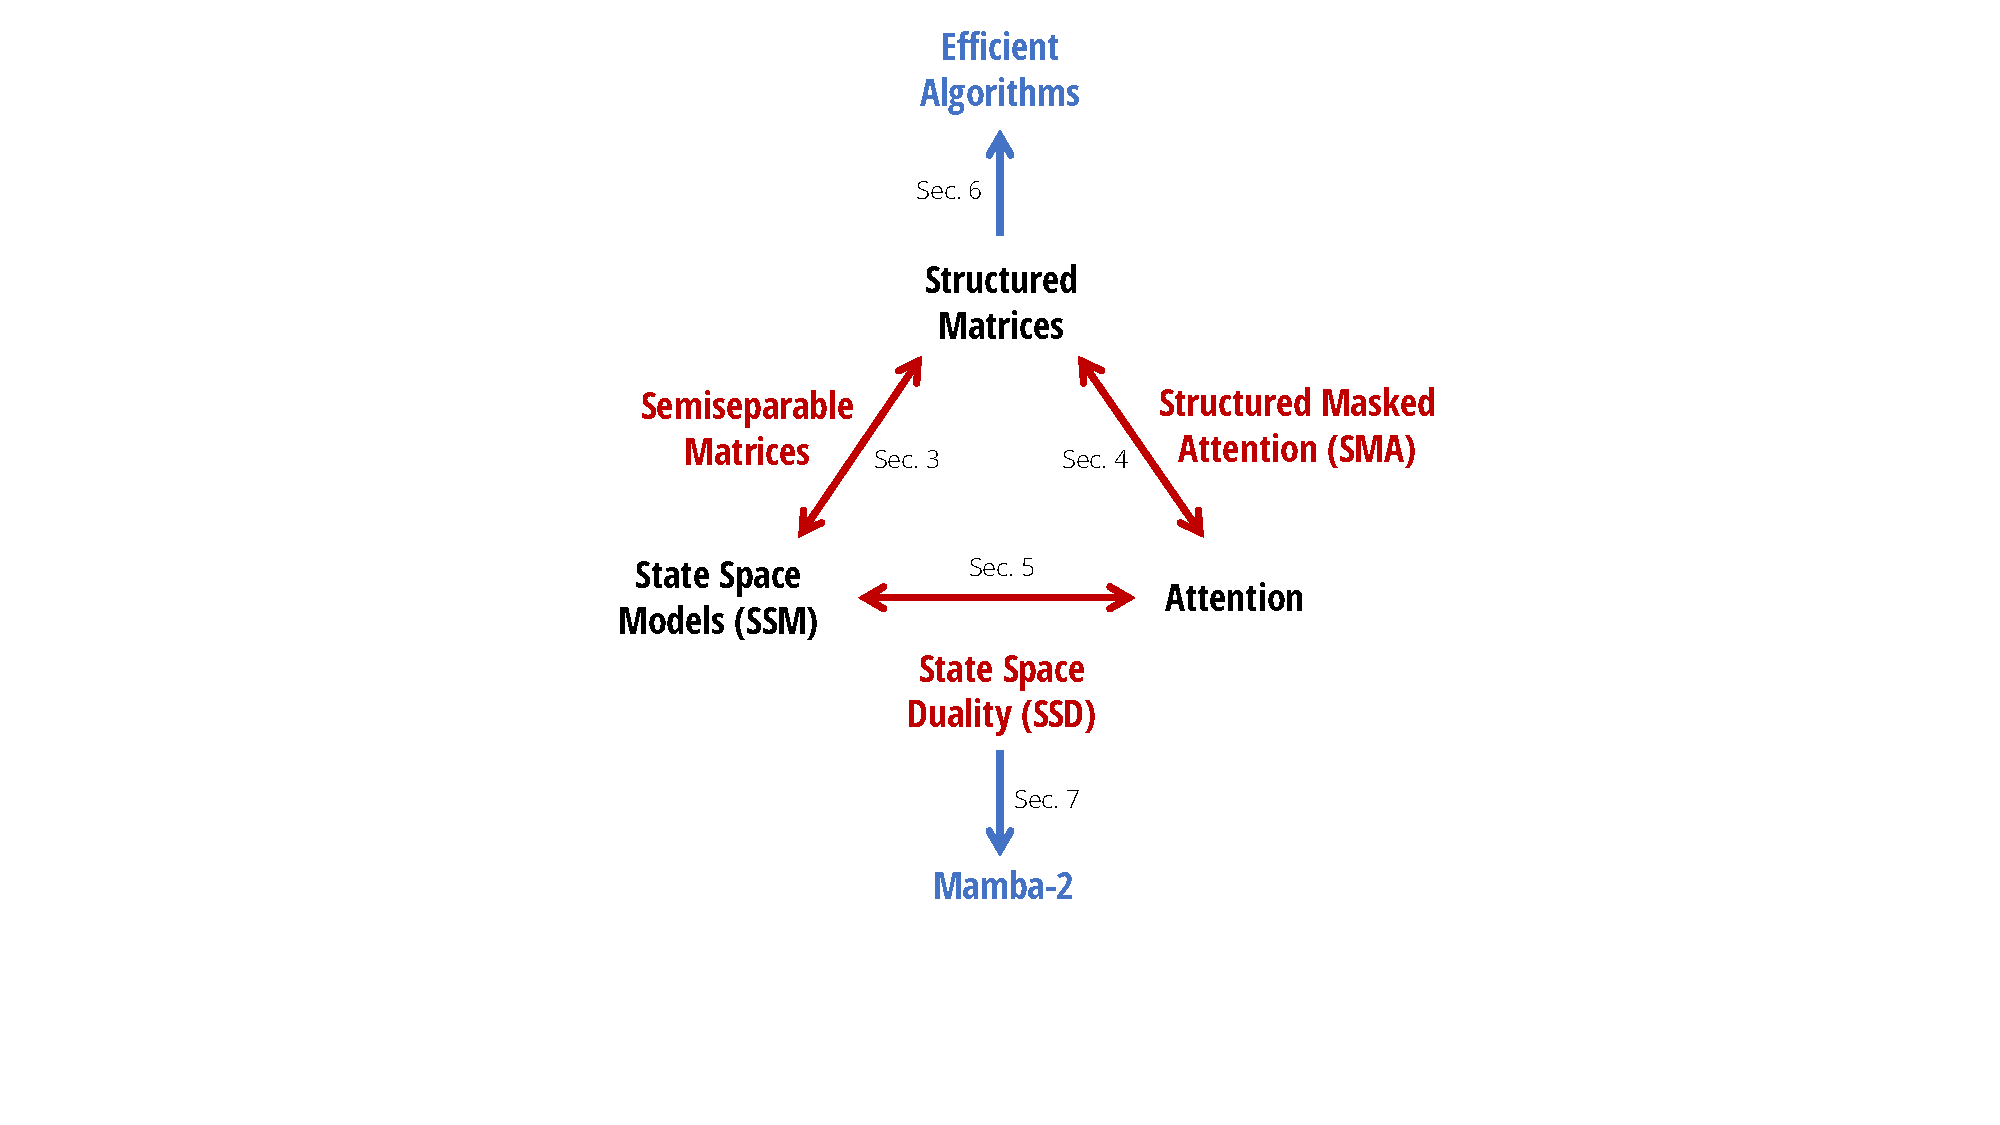
\includegraphics[width=\linewidth]{fig/ssd_roadmap.pdf}
  \end{center}
  \caption{
    (\textbf{Structured State-Space Duality}.)
    This paper fleshes out the relationship between state space models and attention through the bridge of structured matrices.
  }
  \label{fig:roadmap}
\end{wrapfigure}
}{}

\para{State Space Duality.}
Our framework connecting structured SSMs and variants of attention, which we call \textbf{structured state space duality} (SSD),
is made through the abstractions of \textbf{structured matrices}:
matrices with subquadratic parameters and multiplication complexity.
We develop two broad frameworks for representing sequence models, one as matrix transformations and one as tensor contractions, which each reveal different perspectives of the duality.
Our technical contributions include:
\begin{itemize}[leftmargin=*,itemsep=0pt,topsep=0pt]
  \item We show an equivalence between state space models and a well-studied family of structured matrices called \textbf{semiseparable matrices}\iftoggle{arxiv}{ (\cref{sec:ssm})}{}.
    This connection is at the heart our framework, revealing new properties and algorithms for SSMs. A central message of this paper is that \emph{different methods of computing state space models can be reframed as various matrix multiplication algorithms on structured matrices}.
  \item We significantly improve the theory of linear attention~\citep{katharopoulos2020transformers}.
    We first provide an incisive proof of its recurrent form through the language of tensor contractions, and then generalize it to a new family of \textbf{structured masked attention (SMA)}\iftoggle{arxiv}{ (\cref{sec:attention})}{}.
  \item We connect SSMs and SMA, showing that they have a large intersection that are duals of each other, possessing both SSM-like linear and attention-like quadratic forms\iftoggle{arxiv}{ (\cref{sec:ssd})}{}.
    \iftoggle{arxiv}{We also prove that any kernel attention method possessing a fast recurrent form must be an SSM.}{}
\end{itemize}


Beyond its intrinsic theoretical value, our framework opens up a broad set of directions for understanding and improving sequence models.

\para{Efficient Algorithms.}
First and most importantly, our framework exposes new efficient and easily-implementable algorithms for computing SSMs\iftoggle{arxiv}{ (\cref{sec:efficient})}{}.
We introduce a new \textbf{SSD algorithm}, based on block decompositions of semiseparable matrices, that takes advantage of both the linear SSM recurrence and quadratic dual form, obtaining optimal tradeoffs on all main efficiency axes (e.g. training and inference compute, memory usage, and ability to leverage matrix multiplication units on modern hardware).
A dedicated implementation of SSD is $2-8\times$ faster than the optimized selective scan implementation of Mamba, while simultaneously allowing for much larger recurrent state sizes ($8\times$ the size of Mamba or even higher, with minimal slowdown).
SSD is highly competitive with optimized implementations of softmax attention (FlashAttention-2~\citep{dao2023flashattention2}), crossing over at sequence length 2K and 6$\times$ faster at sequence length 16K.


\iftoggle{arxiv}{
\para{Architecture Design.}
One major obstacle to adopting new architectures such as SSMs is the ecosystem tailored to Transformers, such as hardware-efficient optimization and parallelism techniques for large-scale training.
Our framework allows using established conventions and techniques for attention to build a vocabulary of architecture design choices for SSMs, and further improve them (\cref{sec:architecture}).
For example, we introduce the analog of heads from multi-head attention (MHA) to SSMs.
We show that the Mamba architecture is a \textbf{multi-input SSM (MIS)} that turns out to be analogous to \textbf{multi-value attention (MVA)}, and compare other variants of Mamba with different head structures.

We also use these ideas to make slight modifications to the Mamba block, which allows tensor parallelism to be implemented (e.g. in the style of Megatron~\citep{shoeybi2019megatron}).
The main ideas include introducing grouped-value attention (GVA) head structure, and moving all data-dependent projections to occur in parallel at the beginning of the block.


}{
  \para{Mamba-2.}
  Additionally, inspired by the connection between SSMs and Transformers, we slightly modify the neural network architecture of Mamba by moving all data-dependent projections to occur in parallel at the beginning of the block. %
}
The combination of the modified parallel Mamba block, together with using SSD as the inner SSM layer, results in the \textbf{Mamba-2} architecture.
We investigate Chinchilla scaling laws for Mamba-2 in the same setting as Mamba, finding that it Pareto dominates Mamba and Transformer++ in both perplexity and wall-clock time.
We additionally train a family of Mamba-2 models at varying sizes on the Pile, showing that it matches or outperforms Mamba and open source Transformers on standard downstream evaluations.
For example, Mamba-2 with 2.7B parameters trained on 300B tokens on the Pile outperforms Mamba-2.8B, Pythia-2.8B and even Pythia-6.9B trained on the same dataset.

\iftoggle{arxiv}{
\paragraph{Systems Optimizations.}
The SSD framework connects SSMs and Transformers, allowing us to leverage a rich body of work on systems optimizations developed for Transformers~(\cref{sec:systems}).
\begin{itemize}[leftmargin=*,itemsep=0pt,topsep=0pt]
  \item For example, Tensor Parallelism (TP) is an important model parallelism technique to train large Transformer models by splitting each layer across GPUs on the same node.
    We design Mamba-2 to be TP-friendly, reducing the number of synchronization point per block by half.
  \item For very long sequences whose activations do not fit on one device, sequence parallelism has been developed for the attention blocks.
    We describe how to train SSMs in general and Mamba-2 in particular with sequence parallelism, by passing the recurrent states between devices.
  \item For finetuning with examples of different lengths, for best efficiency, Transformer requires sophisticated techniques to remove padding tokens and perform attention on variable length sequences.
    We show how Mamba-2 can be trained with variable sequence lengths efficiently, requiring no padding tokens.
\end{itemize}
}{}

\cref{sec:experiments} empirically validates Mamba-2 on language modeling, training efficiency, and a difficult multi-query associative recall task~\citep{arora2024simple}.
Finally, in \cref{sec:related}, we provide an extended related work and discuss potential research directions opened up by our framework.

Model code and pre-trained checkpoints are open-sourced at \url{https://github.com/state-spaces/mamba}.








% Methods section
%\documentclass[main]{subfiles}

%\begin{document}


\section{Score-based variational inference with orthogonal function expansions}
\label{sec:scorebasedVI}

In this section we use orthogonal function expansions to develop new variational families for
approximate probabilistic inference. In \Cref{sec:orth}, we review the basic properties of these
expansions.
In \Cref{sec:eigenVI}, we introduce a score-based divergence for VI with these families;
notably, for this divergence, the optimization for VI reduces to an eigenvalue
problem. Finally in \Cref{sec:precon},
we consider how to use these variational approximations for unstandardized distributions;
in these settings we must carefully manage the trade-off between expressiveness and
computational~cost.

%%%%%%%%%%%%

\subsection{Orthogonal function expansions}
\label{sec:orth}

Let $\mathcal{Z}\subseteq\mathbb{R}^D$ denote the support of the
target distribution $p$.
Suppose that there exists a
complete set of orthonormal basis functions
$\{\phi_k(z)\}_{k=1}^\infty$ on this set. By \emph{complete}, we mean
that any sufficiently well-behaved function
\mbox{$f:\mathcal{Z}\rightarrow\mathbb{R}$} can be approximated, to
arbitrary accuracy, by a particular weighted sum of these basis
functions, and by \emph{orthonormal}, we mean that the basis functions
satisfy
\begin{align}
\label{eq-orthonormal}
  \int\!\phi_k(z)\phi_{k'}(z)\, dz =
  \left\{
  \begin{array}{rr} 1 & \mbox{if $k=k'$}, \\
    0 & \mbox{otherwise,}\end{array}\right.
\end{align}
where the integral is over $\mathcal{Z}$.
Define the
$K^\text{th}$-order variational family $\mathcal{Q}_K$ to be the set containing
all distributions of the form
\begin{align}
  q(z) =  \left(\sum_{k=1}^{K} \alpha_k \phi_k(z)\right)^2\quad\mbox{where}\quad\sum_{k=1}^{K} \alpha_k^2=1,
\label{eq:OF-1}
\end{align}
and where $\alpha_k\in\R$ for $k=1,\ldots, K$ are the parameters of the family $\mathcal{Q}_K.$
In words,  $\mathcal{Q}_K$ contains all distributions that can be obtained by
taking weighted sums of the first $K$ basis functions and then \textit{squaring} the result.

\Cref{eq:OF-1} involves a squaring operation, a sum-of-squares
constraint, and a weighted sum. The squaring operation ensures that
the density functions in $\mathcal{Q}_K$ are nonnegative (i.e., with
$q(z)\!\geq\!0$ for all $z\in\mathcal{Z}$), while the sum-of-squares constraint
ensures that they are normalized:
\begin{align}
  \int\! q(z)\, dz\, =\, \int\! \left(\sum_{k=1}^{K} \alpha_k \phi_k(z)\right)^2\!\! dz\, =\,
  \int\! \sum_{k,k'=1}^{K} \alpha_k \alpha_{k'} \phi_k(z)\phi_{k'}(z)\, dz\, =\, \sum_{k=1}^{K} \alpha_k^2 = 1.
\end{align}

The weighted sum in \Cref{eq:OF-1} bears a superficial similarity
to a mixture model, but note that neither the basis
functions~$\phi_k(z)$ nor the weights~$\alpha_k$ in \Cref{eq:OF-1}
are constrained to be nonnegative. Distributions of this form arise
naturally in physics from the quantum-mechanical \emph{wave functions}
that satisfy Schr\"odinger's equation \citep{griffiths2018introduction}.
In that setting, though, it is
typical to consider complex-valued weights and basis functions,
whereas here we only consider real-valued ones.


The simplest examples of orthogonal function expansions arise in one
dimension. For example, functions on the interval $[-1,1]$ can be
represented as weighted sums of Legendre polynomials, while functions
on the unit circle can be represented by Fourier series of sines and
cosines; see \Cref{tab:onedim}. Distributions on unbounded
intervals can also be represented in this way. On the real line, for
example, we may consider approximations of the form in
\Cref{eq:OF-1} where
\begin{equation}
\phi_{k+1}(z) = \left(\sqrt{2\pi}k!\right)^{-\frac{1}{2}}\left(e^{-\frac{1}{2}z^2}\right)^{\frac{1}{2}}\,\text{H}_{k}(z),
\label{eq:phi-hermite}
\end{equation}
and $\text{H}_k(z)$ are the \emph{probabilist's} Hermite polynomials given by
\begin{equation}
\text{H}_k(z) = (-1)^k e^{\frac{z^2}{2}} \frac{d^k}{dz^k}\left[e^{-\frac{z^2}{2}}\right].
\label{eq:hermite}
\end{equation}
Note how the lowest-order basis function $\phi_1(z)$ in this family gives rise
(upon squaring) to a Gaussian distribution with zero mean and unit variance.

\Cref{fig:onedim} shows how various multimodal distributions with
one-dimensional support can be approximated by computing weighted sums
of basis functions and squaring their result. We emphasize that
\textit{the more basis functions in the sum, the better the
  approximation}.

%%%%%%%%%%%%

\begin{table*}[t]
\small
%\begin{center}
    \centering
    \caption{Examples of orthogonal function expansions in one dimension. The basis functions in the
        table are not normalized, but they can be rescaled so that their squares integrate to one.
    \vspace{5pt}
    }

    \label{tab:onedim}
    \begin{tabular}{lll}
    \toprule
    \textbf{support} & \textbf{orthogonal family} & \textbf{basis functions} $\phi_k(\cdot)$  \\ [0.3ex]
    \midrule
    $z\in[-1,1]$ & Legendre polynomials & $\{1,\, z,\, 3z^2\!-\!1,\, 5z^3\!-\!3z, \ldots\}$ \\ [0.3ex]
    $z=e^{i\theta}\!\in S^1$\hspace{2ex} & Fourier basis & $\{1,\cos\theta,\sin\theta,\cos 2\theta,\sin 2\theta,\ldots\}$ \\[0.3ex]
    $z\in[0,\infty)$ & weighted Laguerre polynomials &    $e^{-\frac{z}{2}}\{1,1\!-\!z,z^2\!-\!4z\!+\!2,\ldots\}$\\ [-0.3ex]
    $z\in\mathbb{R}$ & weighted Hermite polynomials & $e^{-\frac{z^2}{4}}\{1,z,(z^2\!-\!1),(z^3\!-\!3z),\ldots\}$\\ [0.5ex]
    \bottomrule
    \end{tabular}
    %\end{center}
    \vspace{-10pt}
\end{table*}

\begin{figure}[t]
\centering
\begin{subfigure}[b]{0.325\linewidth}
    \centering
    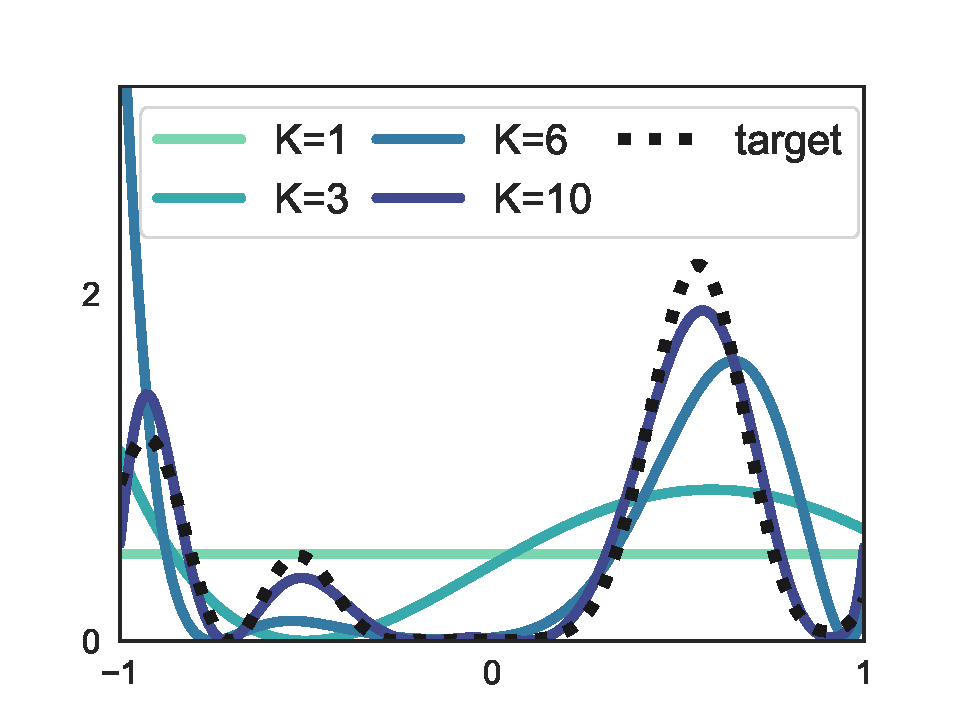
\includegraphics[scale=0.31]{figs/1d_legendre2.pdf}
    \caption{Legendre polynomial expansion}
\end{subfigure}
\begin{subfigure}[b]{0.325\linewidth}
    \centering
    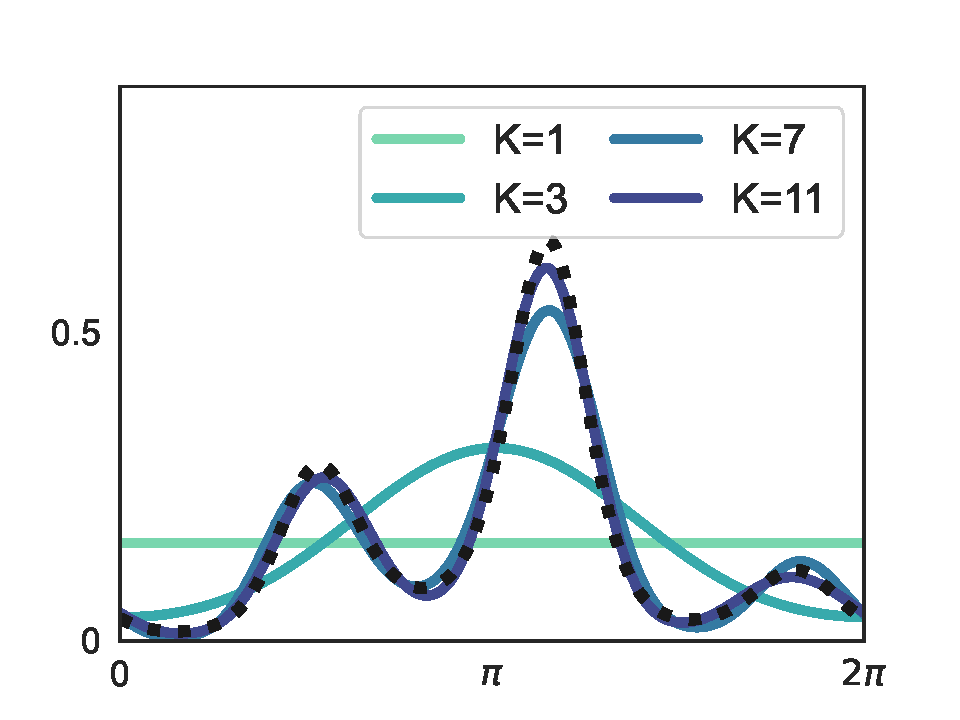
\includegraphics[scale=0.31]{figs/1d_fourier2.pdf}
    \caption{Fourier series expansion}
\end{subfigure}
\begin{subfigure}[b]{0.325\linewidth}
    \centering
    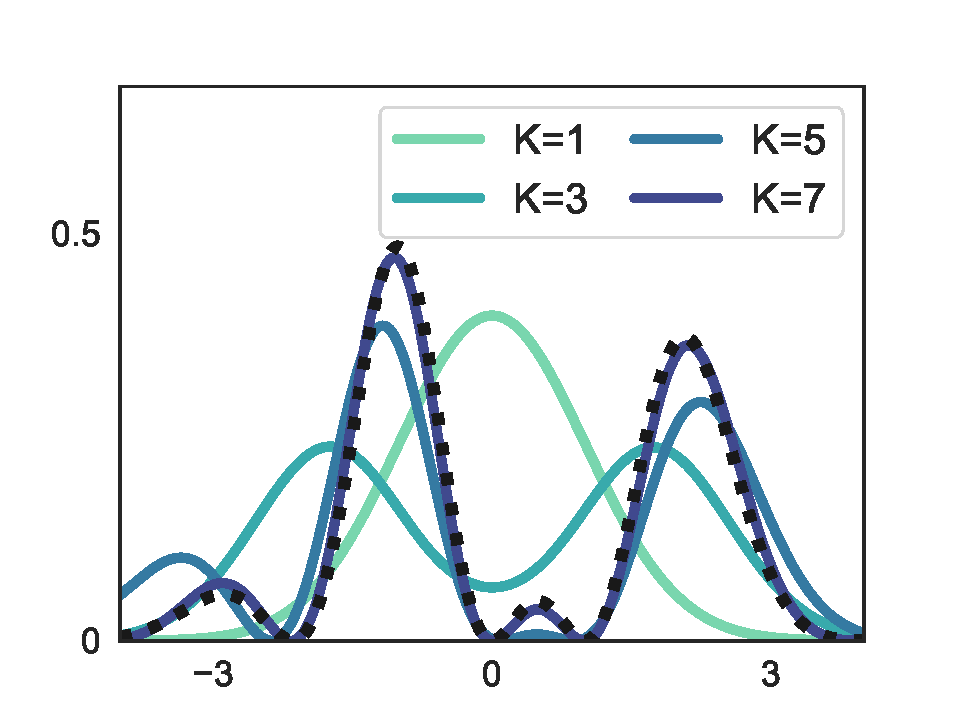
\includegraphics[scale=0.31]{figs/1d_hermite2.pdf}
    \caption{Hermite polynomial expansion}
    \label{fig:onedim:c}
\end{subfigure}
\caption{Target probability distributions (black dashed curves) on the interval $[-1,1]$ (left), the unit circle (middle), and the
    real line (right), and their approximations by orthogonal function expansions
    from different families and of different orders; see \Cref{eq:OF-1} and \Cref{tab:onedim}.}
\vspace{-15pt}
\label{fig:onedim}
\end{figure}

%%%%%%%%%%%%%

Orthogonal function expansions in one dimension are also important because their Cartesian products can be used to generate orthogonal function expansions in higher dimensions. For example, we can approximate distributions over (say) $\mathbb{R}^3$ by
\begin{equation}
q(z_1,z_2,z_3) =  \left(\sum_{i=1}^{K_1}\sum_{j=1}^{K_2}\sum_{k=1}^{K_3} \beta_{ijk}\, \phi_i(z_1)\phi_j(z_2)\phi_k(z_3)\right)^2\quad\mbox{where}\quad \sum_{ijk}\beta^2_{ijk} = 1,
\label{eq:3d}
\end{equation}
where $\beta_{ijk}\in \R$ now parametrize the family.
Note that there are a total $K_1 K_2 K_3$ parameters in the above expansion, so that this method of
Cartesian products does not scale well to high dimensions if multiple basis functions are used per
dimension.
Note that the same strategy can also be used for random variables of
mixed type: for example, from \Cref{tab:onedim}, we can create a variational family of distributions over $\mathbb{R}\!\times\![-1,1]\!\times\![0,\infty)$ from the Cartesian product of orthogonal function expansions involving Hermite, Legendre, and Laguerre polynomials.

As shown in \Cref{fig:onedim}, the approximating distributions
from $K^\text{th}$-order expansions can model the presence of multiple
modes as well as many types of asymmetry, and this expressiveness also
extends to higher dimensions. Nevertheless, it remains tractable to
sample from these distributions and even to calculate (analytically)
their low-order moments, as we show in \Cref{app:sampling,app:moments}.

For concreteness, consider the distribution over $\mathbb{R}^3$ in
\Cref{eq:3d}. The marginal distribution $q(z_1)$ is
\begin{align}
q(z_1) = \int\! q(z_1,z_2,z_3)\,dz_2\, dz_3 = \sum_{ii'} \left[\sum_{jk} \beta_{ijk}\beta_{i'jk}\right] \phi_i(z_1)\phi_{i'}(z_1),
\label{eq:marginal}
\end{align}
and from this expression, moments such as $\mathbb{E}[z_1]$
%(\Cref{eq:Amu})
and
$\text{Var}[z_1]$
%(\Cref{eq:Anu})
can be calculated by evaluating integrals involving
the elementary functions in \Cref{tab:onedim}.
(In practice,
these integrals are further simplified by recursion relations that
relate basis functions of different orders;
we demonstrate how to compute the first two moments for
the normalized Hermite family in
\Cref{eq:mom1ij,eq:mom2ij}.)

To generate samples $\{z^{(t)}\}$, each dimension is sampled as follows:
we draw
$z_1^{(t)} \sim q(z_1)$ by computing the cumulative distribution function (CDF)
of this marginal distribution and then numerically inverting this CDF.
Finally, extending these ideas, we can calculate higher-order moments
and obtain joint samples via the nested draws
\begin{align}
\label{eq:sample}
    z_1^{(t)} \sim q(z_1),\quad z_2^{(t)} \sim q(z_2 \given z_1),\quad
    z_3^{(t)} \sim q(z_3  \given z_1,z_2).
\end{align}
The overall complexity of these procedures scales no worse than
quadratically in the number of basis functions in the expansion. These
extensions are discussed further in \Cref{app:sampling,app:moments}.

%%%%%%%%%%%

\subsection{EigenVI}
\label{sec:eigenVI}

In variational inference, we posit a parameterized family of
approximating distributions and then compute the particular approximation
in this family that is closest to a target distribution of interest.
\Cref{eq:OF-1}
constructs a variational family $\Q_K$ from the orthogonal functions $\{\phi_k(z)\}_{k=1}^K$ whose variational parameters are the weights
$\{\alpha_k\}_{k=1}^{K}$. We now derive \textit{EigenVI}, a method to find
$q \in \Q_K$ that is close to the target distribution $p(z)$.

We first define the measure of closeness that we will minimize.
EigenVI measures the quality of an approximate density by the
\textit{Fisher divergence} \citep{hyvarinen2005estimation},
\begin{align}
\label{eq-divergence}
    \D(q,p) = \int \norm{\nabla \log q(z) - \nabla\log p(z)}^2 q(z) dz,
\end{align}
where $\nabla \log q(z)$ and $\nabla \log p(z)$ are the score functions of the
variational approximation and target, respectively. Suppose that $q$ and $p$ have the same support; then the Fisher divergence vanishes if and only if the scores of $q$ and $p$ are
everywhere equal.

Though $p$ is, by assumption, intractable to compute, in many applications it is
possible to efficiently compute the score $\nabla \log p$ at any point
$z\in\mathcal{Z}$. For example, in Bayesian models the score of the target
posterior is equal to the gradient of the log joint. This observation is the main
motivation for score-based methods in probabilistic
modeling~\citep{liu2016stein,yu2023semiimplicit,modi2023,cai2024}.

Here we seek the $q\!\in\!\Q_K$ that minimizes $\D(q,p)$. But now a
challenge arises: it is generally difficult to evaluate the integral
for $\D(q,p)$ in \Cref{eq-divergence}, let alone to minimize it as a
function of~$q$.
While it is possible to sample from the distribution $q$,
it is not straightforward to simultaneously sample from $q$ and optimize over the variational parameters $\{\alpha_k\}_{k=1}^K$ in terms of which it is defined.
Instead, we construct an unbiased estimator of
$\D(q,p)$ by importance sampling, which also decouples the sampling distribution from the optimization.
Let $\{z^1,z^2,\ldots z^B\}$ denote a
batch of $B$ samples drawn from some proposal distribution $\pi$ on
$\mathcal{Z}$. From these samples we can form the unbiased estimator
\begin{align}
  \label{eq-empirical-divergence}
  \widehat\D_{\pi}(q, p) =
  \sum_{b=1}^B \frac{q(z^b)}{\pi(z^b)} \, \big\|\nabla \log q(z^b) - \nabla\log p(z^b)\big\|^2.
\end{align}
This estimator should be accurate for appropriately broad proposal
distributions and for sufficiently large batch sizes. We can therefore
attempt to minimize \Cref{eq-empirical-divergence} in place of
\Cref{eq-divergence}.

Now we show that the minimization of \Cref{eq-empirical-divergence} over
$q\in\Q_K$ simplifies to a minimum eigenvalue problem for the weights
$\{\alpha_k\}_{k=1}^{K}$.
To obtain the eigenvalue problem, we substitute the
orthogonal function expansion in \Cref{eq:OF-1}
into \Cref{eq-empirical-divergence} for the unbiased estimator of
$\D(q,p)$. As an intermediate step, we differentiate
\Cref{eq:OF-1} to obtain the scores
\begin{equation}
\label{eq:scores}
\nabla\log q(z^b) = \frac{2\sum_k \alpha_k \nabla \phi_k(z^b)}{\sum_k \alpha_k \phi_k(z^b)}.
\end{equation}
Further substitution of the scores provides the key result behind our
approach: the unbiased estimator in
\Cref{eq-empirical-divergence} is a simple quadratic form in the
weights $\alpha := [\alpha_1,\ldots,\alpha_K]^\top$ of the orthogonal function expansion,
\begin{equation}
\widehat\D_{\pi}(q,p) =
\alpha^\top\! M\alpha,
\label{eq:quadform}
\end{equation}
where the coefficients of the quadratic form are given by
\begin{equation} \label{eq:M}
  M_{jk} = \sum_{b=1}^B\frac{1}{\pi(z^b)}
    \left[2\nabla \phi_j(z^b) - \phi_j(z^b)\nabla\log p(z^b)\right]\cdot\left[2\nabla \phi_k(z^b) -
    \phi_k(z^b)\nabla\log p(z^b)\right].
\end{equation}
Note that the elements of the $K\!\times\! K$ symmetric matrix $M$ capture all of the dependence on
the batch of samples $\{z^b\}_{b=1}^B$, the scores of $p$ and $q$ at these samples,
and
the choice of the family of orthogonal functions.
Next we minimize the quadratic
form in \Cref{eq:quadform} subject to the sum-of-squares
constraint $\sum_k \alpha_k^2 = 1$ in \Cref{eq:OF-1}.
In this way we obtain the eigenvalue problem~\citep{courant1924methoden}
\begin{align}
  \label{eq:eigenVI-solution}
\min_{q\in\Q_K}\left[\widehat{\D}_{\pi}(q,p)\right] =
  \min_{\|\alpha\|=1}
  \left[\alpha^\top M\alpha\right] =:
  \lambda_{\text{min}}(M),
\end{align}
where $\lambda_{\text{min}}(M)$ is the minimal eigenvalue of $M$,  and the
optimal weights are given (up to an arbitrary sign) by its
corresponding eigenvector; see \Cref{app:eigen} for a proof.
EigenVI solves \Cref{eq:eigenVI-solution}.

We note that the eigenvalue problem in EigenVI arises from the curious alignment of three particular choices---namely, (i) the choice of variational family
(based on orthogonal function expansions), (ii) the choice of
divergence (based on score-matching), {and (iii) the choice of estimator for the divergence
(based on importance sampling)}.
The simplicity of this eigenvalue problem stands
in contrast to the many heuristics of gradient-based optimizations---involving learning
rates, terminating criteria, and perhaps other algorithmic
hyperparameters---that are typically required for ELBO-based
BBVI~\citep{dhaka2020robust,dhaka2021challenges}.
But EigenVI is also not entirely free of heuristics; to compute the estimator in
\Cref{eq-empirical-divergence} we must also specify the proposal distribution $\pi$ and the number
of samples $B$; see \Cref{sec:discussion:eigenvi} for a discussion.

The size of the eigenvalue problem in EigenVI is equal to the
number of basis functions $K$ in the orthogonal function expansion of \Cref{eq:OF-1}. The
eigenvalue problem also generalizes to orthogonal function expansions
that are formed from Cartesian products of one-dimensional families,
but in this case, if multiple basis functions are used per dimension,
then the overall basis size grows exponentially in the dimensionality.
Thus, for example, the eigenvalue problem would be of size
$K_1 K_2 K_3$ for the approximation in \Cref{eq:3d}, as can be
seen by ``flattening'' the tensor of weights $\beta$ in \Cref{eq:3d}
into the vector of weights $\alpha=\textbf{vec}(\beta)$ in \Cref{eq:OF-1}.
Finally, we note that EigenVI only needs to compute the minimal eigenvector of $M$ in \Cref{eq:eigenVI-solution}, and therefore it can benefit from specialized routines that are much less expensive than a full diagonalization.




\subsection{EigenVI in $\reals^D$:\ the Hermite family and standardization}
\label{sec:precon}

We now discuss the specific case of EigenVI for $\mathcal{Z}\!=\!\reals^D$ with the Hermite-based variational family in \Cref{eq:phi-hermite}.
For this case, we propose a transformation of the domain that serves to precondition or \textit{standardize}
the target distribution before applying EigenVI.
While this standardization is not required to use EigenVI,
it  helps to reduce the number of basis functions needed to approximate the target,
leading to a more computationally efficient procedure.
It also suggests natural default choices for the
proposal distribution $\pi$ in \Cref{eq-empirical-divergence}.

Recall that the eigenvalue problem grows linearly in size with the number of basis functions. Before applying EigenVI, our goal is therefore to transform the domain in a way that reduces the number of basis functions needed for a good approximation.
To meet this goal for distributions over $\reals^D$, we observe that the lowest-order basis function of the Hermite family in \Cref{eq:phi-hermite} yields (upon squaring) a standard multivariate Gaussian, with zero mean and unit covariance.
Intuitively, we might expect the approximation of EigenVI to require fewer basis functions if the statistics of the target distribution nearly match those of this lowest-order basis function. The goal of standardization is to achieve this match, to whatever extent possible, by a suitable transformation of the underlying domain. Having done so, EigenVI in $\reals^D$ can then be viewed as
a systematic framework to model non-Gaussian effects via a small number of higher-order terms in its orthogonal function expansion.

Concretely, we consider a linear transformation  of the domain:
\begin{align}
    \tilde{z} =
    %\T(z) =
    \Sigma^{-\frac{1}{2}}(z\!-\!\mu),
\end{align}
where $\mu$ and $\Sigma$ are  estimates of the mean and covariance
obtained
from some other algorithm
(e.g., a Laplace approximation,  Gaussian variational inference,  Monte Carlo, or domain-specific
knowledge).
We then apply the EigenVI to fit a $K$th-order variational approximation $\tilde q(\tilde z)$
to the target distribution $\tilde{p}(\tilde{z})$ that is induced by this transformation;
afterwards, we reverse the change-of-variables to obtain the final approximation to $p(z)$, i.e.,
\begin{align}
q(z) = \tilde{q}(\tilde{z})|\Sigma|^{-1/2}.
\end{align}

\Cref{fig:standardize} shows why it is more difficult to approximate distributions that are
badly centered or poorly scaled. The left panel shows the effect of translating a standard Gaussian
\textit{away} from the origin and \textit{shrinking} its variance; note how a comparable
approximation to the uncentered Gaussian now requires a 16th-order expansion.
On the other hand, after standardization, the target
can be perfectly fitted by the base distribution
in the orthogonal family of reweighted Hermite polynomials.
%
The right panel shows
the similar effect of translating the mixture distribution in \Cref{fig:onedim} (right panel);
comparing these panels, we see that twice as many basis functions ($K\!=\!14$ versus $K\!=\!7$)
are required to provide a comparable fit of the uncentered mixture.


\begin{figure}
\centering
\begin{subfigure}[b]{0.40\linewidth}
    \centering
    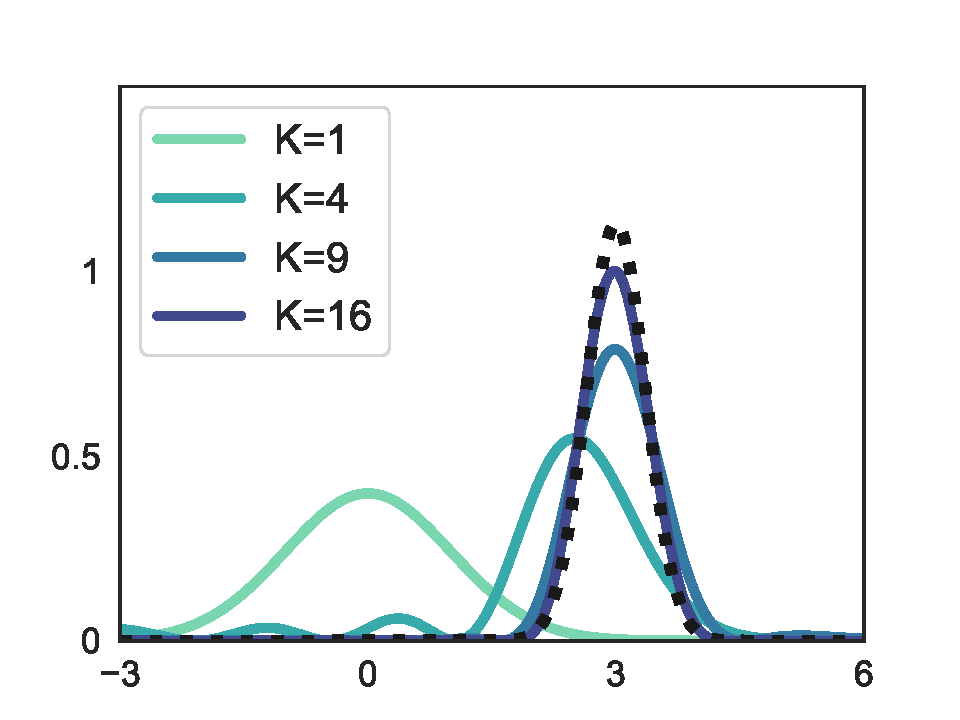
\includegraphics[scale=0.31]{figs/1d_precond_gauss2.pdf}
    \caption{Gaussian target, mean $3$ and variance $\frac{1}{8}$}
\end{subfigure}
\begin{subfigure}[b]{0.40\linewidth}
    \centering
    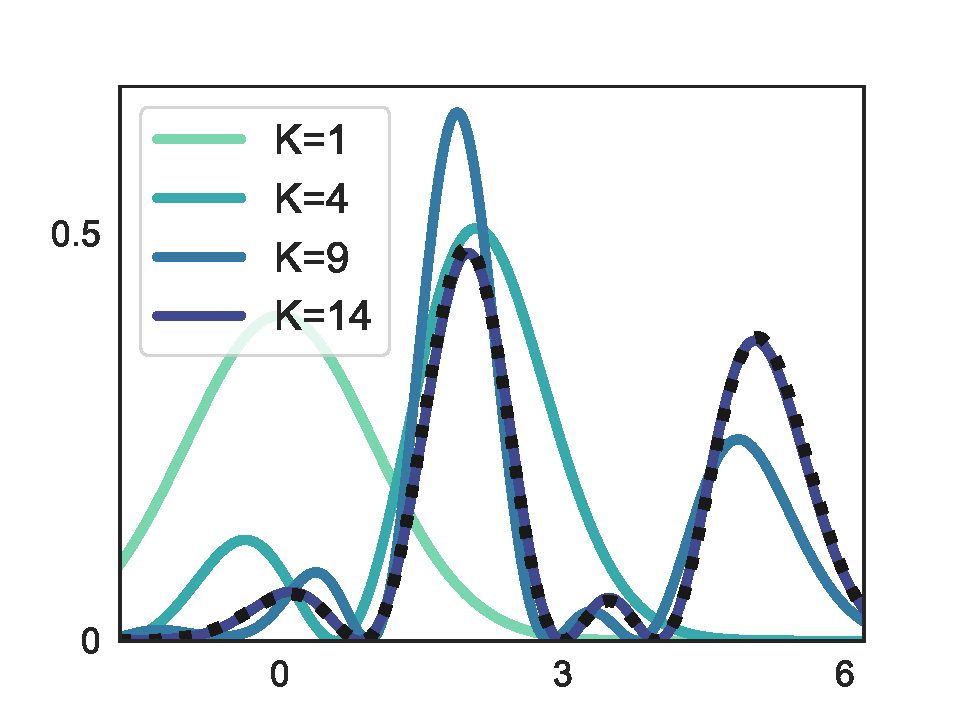
\includegraphics[scale=0.31]{figs/1d_precond_mixture2.pdf}
\caption{Mixture target (translation of \Cref{fig:onedim:c})}
\end{subfigure}
    \caption{Higher-order expansions may be required to approximate target distributions
(black)
    that are not standardized. \textit{Left:} approximation of a non-standardized Gaussian.
    \textit{Right:} approximation of the mixture distribution
    in \Cref{fig:onedim} after translating its largest modes away from the origin.
}
\label{fig:standardize}
\vspace{-13pt}
\end{figure}

Finally, we note another benefit of standardizing the target before fitting EigenVI; when the target has nearly zero mean and unit covariance, it becomes simpler to identify natural choices for the proposal distribution $\pi$.
Intuitively, in this case, we want a proposal distribution that has the same mean but heavier tails than a standard Gaussian.
In our experiments, we use two types of centered proposal distributions---uniform and isotropic Gaussian---whose variances are greater than one.


%\end{document}


%%% Local Variables:
%%% mode: latex
%%% TeX-master: "main"
%%% End:


% Other related work
\section{Related work}

There is a rich prior literature on 
probabilistic programming languages (PPLs),
which extend probabilistic graphical models to
support more complex joint distributions whose size and ``shape''
can itself be stochastic (e.g., a graph
unrolled for a random number of iterations,
until a data-dependent stopping criterion is met).
PPLs extend traditional programming languages with the ability to {\it sample} from distributions and {\it observe} values of variables based on data (i.e. condition the model).
The semantics of sample and observe vary depending on the inference algorithm.
For more details, see  \citet{intro_ppl}.

Recently there has been an explosion of interest in large language models, such as 
GPT-3 \citep{gpt3} and PaLM \citep{palm}.
%\citep{lamda}.
These can be used for tasks such as ``zero-shot"
question-answering. In this setting, we 
provide the question $Q$ as a prompt to the LM,
and then sample answers from the model, 
which we denote by $p(A|Q,\theta)$,
where $\theta$ are the pre-trained model parameters.
Alternatively, we can compute the MAP answer,
$\hat{A} = \argmax_A p(A|Q,\theta)$.


To ensure the model ``does the right thing'',
we can provide a small training set of question-answer pairs,
$D = \{ (Q^m,A^m): m=1:M\}$ pairs.
This can be provided as extra context to the model,
provided in the text prompt, followed by sampling
from $p(A|Q,D,\theta)$.
We refer to this as ``few-shot prompting''.
We can also fine-tune the model parameters on $D$ to
get $\theta'$, and then sample
from $p(A|Q,\theta')$.

%We can improve performance on question answering tasks by encouraging the model
%chaining multiple LMs together,  % david: They don't actually do multiple calls, just prompt it to produce the aux variable directly.
%as illustrated in the
%Scratchpad \citep{scratchpads} and Chain of Thought \citep{chainofthought}  papers.
%These papers introduce an  an additional auxiliary ``thought''
%variable $T$ and then extend the model to have the form
%$P(A,T|Q) = P(A|T,Q)P(T|Q)$, where each conditional is computed
%using an LM.

We can improve performance by introducing an additional auxiliary ``thought'' variable,
and then extend the model to have the form $p(A,T|Q) = p(A|T,Q)p(T|Q)$, where each conditional is computed using an LM which includes its conditioning variables as a part of its input.
Work on scratchpads \citep{scratchpads} and chain of thought \citep{chainofthought} illustrate this, and finetune or prompt the LM to produce this auxiliary thought before answering.
%We can improve performance on question answering tasks by encouraging the model
%chaining multiple LMs together,  % david: They don't actually do multiple calls, just prompt it to produce the aux variable directly.
% These papers 
% variable $T$ 

We typically condition this on a small set
$D_S$ of  $(A^m,T^m,Q^m)$ triples,
and optionally a larger set $D_L$ of $(A^m, Q^m)$ pairs.
We then compute a distribution over answers to a test question
using
\begin{align}
\hat{p}(A|Q) = \sum_T 
\hat{p}(A|Q, T) \hat{p}(T|Q)
\label{eqn:probQA}
\end{align}
where $\hat{p}(\cdot) = p(\cdot|D_L,D_S,\theta)$
is the prior predictive distribution. (Scratchpad creates its prior predictive by fine-tuning, while Chain of Thought adds $D_S$ to the LM prompt.)

In practice, we cannot sum over all possible strings $T$
in \cref{eqn:probQA}.
The most common approach is to compute the MAP estimate
$\hat{T} = \argmax \hat{p}(T)$ using beam search,
and then to approximate the sum over $T$ with this single
value.
More recently, Self Consistency \citep{selfconsistency} 
proposed to sample multiple values for $T$
using forward sampling of $(A,T)$ given $Q$,
and then taking the answer $A$ that is most common
in this set\footnote{This bucketing is practical because most standard benchmarks have answers that are just a couple words.}.

PromptChainer \citep{promptchainer} proposes a visual interface for composing language models together, specifying control flow and prompting strategies for each node in a chain. Nodes may query language models or external systems. 
Socratic models \citep{socraticmodels} extends model chaining to the multimodal setting and demonstrates zero-shot abilities on tasks for which no single model exists.

The Eliciting Latent Knowledge proposal \citep{ELK} suggests making latent variables explicit, modelled using a Bayesian network, to improve interpretability and safety for advanced AI systems.
% Factored cognition \citet{factored_cognition}

\citet{ortega2021shaking} explains a formalism for LM finetuning with causal graphical models in order to extend the predictive capabilities of AI agents towards more adaptive behaviour. They focus on analysing an auto-regressive action (random variable) prediction scheme in the interactive setting of RL where a model is simultaneously a generator and predictor of data.

% \citet{language_feedback} incorporates language feedback to finetune models, and finds that learning is significantly more sample efficient. \ddohan{We view this feedback as an auxiliary variable which can be conditioned to inform inference.}

%\kevin{Omit RL refs since not relevant?}
%Incorporating human feedback into generative models remains an open problem. Reinforcement from human feedback has become a popular approach to finetuning models against human preferences. \citep{learning_to_summarize, anthropic_human_feedback} learn a surrogate model of human preferences and use PPO \citep{ppo} to finetune a language model to maximize this surrogate. Rather than using scalar feedback, \citet{language_feedback} incorporates language feedback to finetune models, and finds that learning is significantly more sample efficient. \ddohan{We view this feedback as an auxiliary variable which can be conditioned to inform inference.}
%\todo{ddohan: consider adding back in language feedback ref}

%\citep{Levine2022} presents some very recent work on using frozen LMs in various ways.\rif{Suggest we cut this if we don't have more to say.}







% Experiments
\vspace{-0.2cm}
\section{Experiments Details}
\label{sec:exp}

\vspace{-0.2cm}
\subsection{Roadmap Insights on FFHQ-256\texorpdfstring{~\cite{sg1}}{}}
\label{sub:arc-experiments}
\vspace{-0.1cm}
As per Table~\ref{tab:roadmap}, Config A (vanilla StyleGAN2) achieves an FID of 7.52 using the official implementation on FFHQ-256. Config B with all tricks removed achieves an FID of 12.46---performance drops as expected. 
Config C, with a well-behaved loss, achieves an FID of 11.65. But, now training is sufficiently stable to improve the architecture.

Config D, which improves $G$ and $D$ based on the classic ResNet and ConvNeXt findings, achieves an FID of 9.95. The output skips of the StyleGAN2 generator are no longer useful given our new architecture; including them produces a worse FID of 10.17. Karras~\etal find that the benefit of output skips is mostly related to gradient magnitude dynamics~\cite{sg3}, and this has been addressed by our ResNet architecture. For StyleGAN2, Karras~\etal conclude that a ResNet architecture is harmful to $G$~\cite{sg2}, but this is not true in our case as their ResNet implementation is considerably different from ours: 1) Karras~\etal use one 3-3 residual block for each resolution stage, while we have a separate transition layer and two 1-3-1 residual blocks; 2) i.3) and i.4) are violated as they do not have a linear residual block~\cite{mobnet} and the transition layer is placed on the skip branch of the residual block rather than the stem; 3) the essential principle of ResNet~\cite{resnet}---identity mapping~\cite{resnet2}---is violated as Karras~\etal divide the output of the residual block by $\sqrt{2}$ to avoid variance explosion due to the absence of a proper initialization scheme.

For Config E, we conduct two experiments that ablate i.\ref{item:i1} (increased width with depthwise conv.) and i.\ref{item:i2} (an inverted bottleneck). We add GroupedConv and reduce the bottleneck compression ratio to two given the same model size. Each bottleneck is now 1.5$\times$ the width of Config A, and the FID drops to 7.51, surpassing the performance of StyleGAN2. By inverting the stem and the bottleneck dimensions to enhance the capacity of GroupedConv, our final model achieves an FID of 7.05, exceeding StyleGAN2.


\begin{wraptable}[12]{r}{6.5cm}
\vspace{-1.25cm}
\centering
\caption{StackedMNIST 1000-mode coverage.}
% Our model outperforms other GANs in terms of $D_\text{KL}$, indicating that we are better able to recover the distribution.}
\vspace{-0.4cm}
\resizebox{0.8\linewidth}{!}{
\begin{tblr}{
  cell{2}{2} = {c},
  cell{2}{3} = {c},
  cell{3}{2} = {c},
  cell{3}{3} = {c},
  cell{4}{2} = {c},
  cell{4}{3} = {c},
  cell{5}{2} = {c},
  cell{5}{3} = {c},
  cell{6}{2} = {c},
  cell{6}{3} = {c},
  cell{7}{2} = {c},
  cell{7}{3} = {c},
  cell{8}{2} = {c},
  cell{8}{3} = {c},
  cell{9}{2} = {c},
  cell{9}{3} = {c},
  cell{10}{2} = {c},
  cell{10}{3} = {c},
  cell{11}{2} = {c},
  cell{11}{3} = {c},
  cell{12}{2} = {c},
  cell{12}{3} = {c},
  hline{2,12} = {1-3}{},
}
Model     & \# modes$\uparrow$ & $D_\text{KL}$$\downarrow$            &  \\
DCGAN~\cite{dcgan}     & 99            & 3.40\phantom{0}&  \\
VEEGAN~\cite{srivastava2017veegan}    & 150           & 2.95\phantom{0}&  \\
WGAN-GP~\cite{wgan-gp}& 959           & 0.73\phantom{0}&  \\
PacGAN~\cite{pacgan}    & 992           & 0.28\phantom{0}&  \\
StyleGAN2~\cite{sg2} & 940           & 0.42\phantom{0}&  \\
PresGAN~\cite{presgan}   & \textbf{1000} & 0.12\phantom{0}&  \\
Adv. DSM~\cite{advsm}  & \textbf{1000} & 1.49\phantom{0}&  \\
VAEBM~\cite{vaebm}     & \textbf{1000} & 0.087          &  \\
DDGAN~\cite{ddgan}     & \textbf{1000} & 0.071          &  \\
MEG~\cite{meg}       & \textbf{1000} & 0.031          &  \\
Ours---Config E     & \textbf{1000} & \textbf{0.029} &  
\end{tblr}
}
\label{tab:stackedmnist}
\end{wraptable}%

\subsection{Mode Recovery --- StackedMNIST\texorpdfstring{~\cite{metz2016unrolled}}{}} 
\vspace{-0.1cm}
We repeat the earlier experiment in 1000-mode convergence on StackedMNIST (unconditional generation), but this time with our updated architecture and with comparisons to SOTA GANs and likelihood-based methods (Tab.~\ref{tab:stackedmnist}, Fig.~\ref{fig:stacked-mnist}). 
One advantage brought up of likelihood-based models such as diffusion over GANs is that they achieve mode coverage~\cite{adm}. We find that most GANs struggle to find all modes. But, PresGAN~\cite{presgan}, DDGAN~\cite{ddgan}, and our approach are successful. Further, our method outperforms all other tested GAN models in term of KL divergence.

\subsection{FID --- FFHQ-256\texorpdfstring{~\cite{sg1}}{} (Optimized)}
\vspace{-0.1cm}
We train Config E model until convergence and with optimized hyperparameters and training schedule on FFHQ at 256$\times$256 (unconditional generation) (Tab.~\ref{tab:ffhq256}, Figs.~\ref{fig:ffhq-256-teaser} and~\ref{fig:ffhq-256}). 
Please see our supplemental material for training details.
%The hyperparameters and schedule are listed in the supplemental material. 
Our model outperforms existing StyleGAN methods, plus four more recent diffusion-based methods. On this common dataset experimental setting, many methods (not listed here) use the bCR~\cite{zhao2021improved} trick---this has only been shown to improve performance on FFHQ-256 (not even at different resolutions of FFHQ)~\cite{zhao2021improved, zhang2022styleswin}. We do not use this trick. 
% no such tricks in our method.
% JT Try to minimize embellishment...
% This is particularly impressive given the fact that the dataset FFHQ was designed for StyleGAN~\cite{sg1} and the StyleGAN series of models were optimized with this specific dataset in mind.
% to achieve this performance.

\subsection{FID --- FFHQ-64\texorpdfstring{~\cite{edm}}{}}
\vspace{-0.1cm}
To compare with EDM~\cite{edm} directly, we evaluate our model on FFHQ at 64$\times$64 resolution. For this, we remove the two highest resolution stages of our 256$\times$256 model, resulting in a generator that is less than half the number of parameters as EDM. Despite this, our model outperforms EDM on this dataset and needs one function evaluation only (Tab.~\ref{tab:ffhq64}).

\begin{figure}
\begin{floatrow}
    %\hspace{-0.75cm}%
    \capbtabbox{%
        \centering
        \resizebox{\linewidth}{!}{
        \begin{tblr}{
          column{2,3} = {r},
          cell{1}{2} = {c},
          cell{1}{3} = {c},
          hline{2,5,9,10} = {-}{},
        }
        Model       & NFE$\downarrow$ & FID$\downarrow$  \\
        StyleGAN2~\cite{sg2}   & 1               & 3.78 \\
        StyleGAN3-T~\cite{sg3} & 1               & 4.81 \\
        StyleGAN3-R~\cite{sg3} & 1               & 3.92 \\
        LDM~\cite{rombach2022high} & 200               & 4.98\\
        ADM (DDIM)~\cite{adm,compdiff} & 500               & 8.41\\
        ADM (DPM-Solver)~\cite{adm,compdiff} & 500               & 8.40\\
        Diffusion Autoencoder~\cite{diffae,compdiff} & 500               & 5.81\\
        Ours---Config E  & 1               & 2.75 \\
        \emph{With ImageNet feature leakage~\cite{kynkaanniemi2022role}:} & & \\
        PolyINR*~\cite{singh2023polynomial} & 1               & 2.72 \\
        StyleGAN-XL*~\cite{sgxl} & 1               & 2.19 \\
        StyleSAN-XL*~\cite{takida2024san} & 1               & 1.68 \\
        \end{tblr}
        }
    }{%
        \caption{
        \label{tab:ffhq256}FFHQ-256. * denotes models that leak ImageNet features.}
    }
    %
    \capbtabbox{%
        \centering
        \resizebox{0.85\linewidth}{!}{
        \begin{tblr}{
          column{2} = {r},
          column{3} = {r},
          hline{2,5,8} = {-}{},
        }
        Model         & NFE$\downarrow$ & FID$\downarrow$ \\
        StyleGAN2~\cite{sg2,anycostgan}     & 1               & 3.32            \\
        MSG-GAN~\cite{karnewar2020msg,anycostgan}       & 1               & 2.7             \\
        Anycost GAN~\cite{anycostgan}   & 1               & 2.52            \\
        VE~\cite{sde,edm}            & 79              & 25.95           \\
        VP~\cite{sde,edm}            & 79              & 3.39            \\
        EDM~\cite{edm}           & 79              & 2.39            \\
        Ours—Config E & 1               & 1.95 \\
        \end{tblr}
        }
    }{%
        \caption{\label{tab:ffhq64}FFHQ-64.}
    }
\end{floatrow}
\vspace{-0.25cm}
\end{figure}


% \begin{figure}
% \begin{floatrow}
%     \capbtabbox{%
%         \centering
%         \resizebox{0.8\linewidth}{!}{
%         \begin{tblr}{
%           column{2,3} = {r},
%           cell{1}{2} = {c},
%           cell{1}{3} = {c},
%           hline{2,9,13} = {-}{},
%         }
%         Model               & NFE$\downarrow$ & FID$\downarrow$ \\
%         BigGAN~\cite{biggan}              & 1               & 14.73 \\
%         TransGAN~\cite{trans}            & 1               & 9.26 \\
%         ViTGAN~\cite{vitgan}              & 1               & 6.66 \\
%         DDGAN~\cite{ddgan}               & 4               & 3.75 \\
%         Diffusion StyleGAN2~\cite{diffusiongan} & 1               & 3.19 \\
%         StyleGAN2 + ADA~\cite{sg2ada}     & 1               & 2.42 \\
%         StyleGAN3-R + ADA~\cite{sg3,studio}   & 1               & 10.83 \\
%         DDPM~\cite{ddpm}               & 1000            & 3.21 \\
%         DDIM~\cite{ddim}                & 50             & 4.67 \\
%         VE~\cite{sde,edm}                  & 35              & 3.11 \\
%         VP~\cite{sde,edm}                  & 35              & 2.48 \\
%         Ours---Config E     & 1               & 1.96 \\
%         \hline
%         \emph{With ImageNet feature leakage~\cite{kynkaanniemi2022role}:} & & \\
%         StyleGAN-XL*~\cite{sgxl}       & 1               & 1.85 \\
%         \end{tblr}
%         }
%     }{%
%         \caption{\label{tab:cifar10}CIFAR-10.}
%     }
%         % \begin{tblr}{
%         %   column{2,3} = {r},
%         %   cell{1}{2}{3} = {},
%         %   hline{2,9,13} = {-}{},
%         % }
%         % Model               & FID$\downarrow$ & Params          \\
%         % BigGAN~\cite{biggan}              & 14.73  & --       \\
%         % TransGAN~\cite{trans}            & 9.26 & --         \\
%         % ViTGAN~\cite{vitgan}              & 6.66 & --         \\
%         % DDGAN~\cite{ddgan}               & 3.75 & --         \\
%         % Diffusion StyleGAN2 & 3.19 & 40.1M           \\
%         % StyleGAN2 + ADA     & 2.42 & 40.1M          \\
%         % StyleGAN3-R + ADA   & 10.83 & 40.1M        \\
%         % DDPM               & 3.21 & 35.2M         \\
%         % DDIM                & 4.67 & --         \\
%         % VE~\cite{edm}                  & 3.11 & 61.8M        \\
%         % VP~\cite{edm}                  & 2.48 & 61.8M         \\
%         % Ours---Config E     & \textbf{1.99}  & 43.0M \\
%         % StyleGAN-XL*~\cite{sgxl}       & 	1.85 & 140.0M \\
%         % \end{tblr}
        
%     %     }
%     % }{%
%     %     \caption{\label{tab:cifar10}CIFAR-10.}
%     % }%
%     %\hspace{-0.75cm}%
%     %\hspace{-0.5cm}%
% \end{floatrow}
% \end{figure}

\subsection{FID --- CIFAR-10~\cite{krizhevsky2009learning}} \vspace{-0.1cm}

\begin{wraptable}[14]{r}{6.5cm}
\vspace{-0.75cm}
\centering
\caption{\label{tab:cifar10}CIFAR-10 performance.}
\vspace{-0.4cm}
\resizebox{0.9\linewidth}{!}{
    \begin{tblr}{
          column{2,3} = {r},
          cell{1}{2} = {c},
          cell{1}{3} = {c},
          hline{2,9,13} = {-}{},
        }
        Model               & NFE$\downarrow$ & FID$\downarrow$ \\
        BigGAN~\cite{biggan}              & 1               & 14.73 \\
        TransGAN~\cite{trans}            & 1               & 9.26 \\
        ViTGAN~\cite{vitgan}              & 1               & 6.66 \\
        DDGAN~\cite{ddgan}               & 4               & 3.75 \\
        Diffusion StyleGAN2~\cite{diffusiongan} & 1               & 3.19 \\
        StyleGAN2 + ADA~\cite{sg2ada}     & 1               & 2.42 \\
        StyleGAN3-R + ADA~\cite{sg3,studio}   & 1               & 10.83 \\
        DDPM~\cite{ddpm}               & 1000            & 3.21 \\
        DDIM~\cite{ddim}                & 50             & 4.67 \\
        VE~\cite{sde,edm}                  & 35              & 3.11 \\
        VP~\cite{sde,edm}                  & 35              & 2.48 \\
        Ours---Config E     & 1               & 1.96 \\
        \hline
        \emph{With ImageNet feature leakage~\cite{kynkaanniemi2022role}:} & & \\
        StyleGAN-XL*~\cite{sgxl}       & 1               & 1.85 \\
        \end{tblr}
}
\end{wraptable}

We train Config E model until convergence and with optimized hyperparameters and training schedule on CIFAR-10 (conditional generation) (Tab.~\ref{tab:cifar10}, Fig.~\ref{fig:cifar10}). Our method outperforms many other GANs by FID even though the model has relatively small capacity. For instance, StyleGAN-XL~\cite{sgxl} has 18\ M parameters in the generator and 125\ M parameters in the discriminator, while our model has a 40\ M parameters between the generator and discriminator combined (Fig.~\ref{fig:fid-50k-vs-params-cifar-10}). Compared to diffusion models like LDM or ADM, GAN inference is significantly cheaper as it requires only one network function evaluation compared to the tens or hundreds of network function evaluations for diffusion models without distillation. 

\begin{wrapfigure}[12]{r}{6.5cm}
    \vspace{-0.4cm}
    \centering
    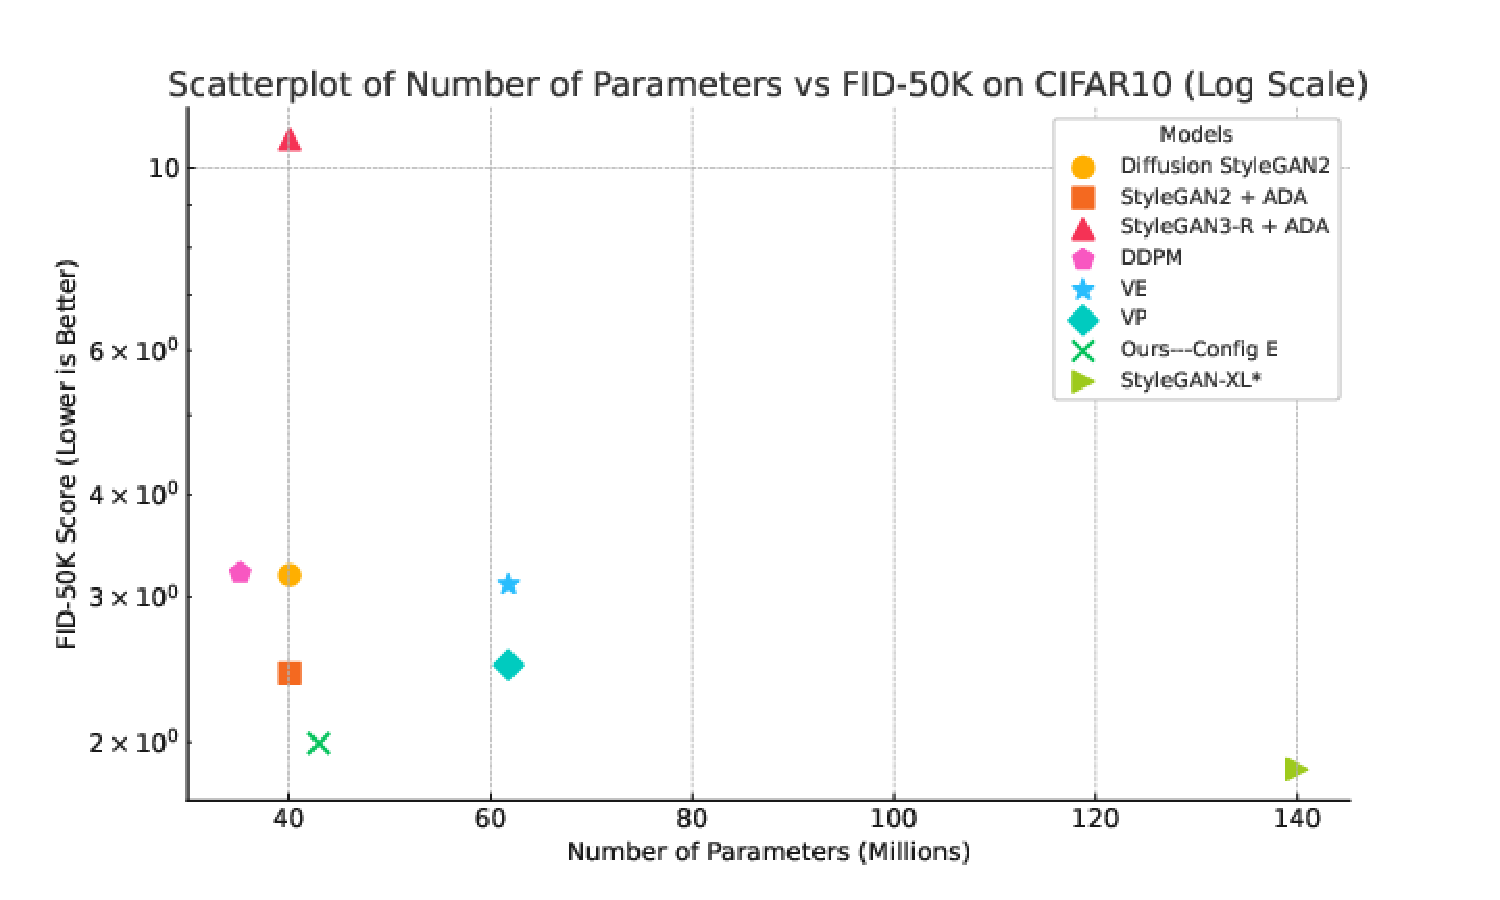
\includegraphics[width=\linewidth,clip,trim={0 0 0 2cm}]{figures/Scatterplot-FID-Parameters-CIFAR10.pdf}
    \caption{Millions of parameters vs.~FID-50K (log scale) on CIFAR-10. Lower is better.}
    \label{fig:fid-50k-vs-params-cifar-10}
\end{wrapfigure}

Many state-of-the-art GANs are derived from Projected GAN~\cite{sauer2021projected}, including StyleGAN-XL~\cite{sgxl} and the concurrent work of StyleSAN-XL~\cite{takida2024san}. These methods use a pre-trained ImageNet classifier in the discriminator. Prior work has shown that a pre-trained ImageNet discriminator can leak ImageNet features into the model~\cite{kynkaanniemi2022role}, causing the model to perform better when evaluating on FID since it relies on a pre-trained ImageNet classifier for the loss. But, this does not improve results in perceptual studies~\cite{kynkaanniemi2022role}. Our model produces its low FID without any ImageNet pre-training.

%\jt{Missing citations here for such methods.}


%\aaron{add NFEs}
%\jt{Which models in our evaluation use this? Any?}

%\jt{What is the second caveat?}

\subsection{FID --- ImageNet-32~\cite{chrabaszcz2017downsampled}}
\label{sec:imagenet32-fid-explain}
We train Config E model until convergence and with optimized hyperparameters and training schedule on ImageNet-32 (conditional generation). We compare against recent GAN models and recent diffusion models in Table~\ref{tab:imagenet32}.
We adjust the number of parameters in the generator of our model to match StyleGAN-XL~\cite{sgxl}'s generator (84M parameters). Specifically, we make the model significantly wider to match. Our method achieves comparable FID despite using a 60\% smaller discriminator (Tab.~\ref{tab:imagenet32}) and despite not using a pre-trained ImageNet classifier.
%, which has been shown to improve FID performance, but not improve results in perceptual studies~\cite{kynkaanniemi2022role}.

\vspace{-0.1cm}
\subsection{FID --- ImageNet-64~\cite{chrabaszcz2017downsampled}}
We evaluate our model on ImageNet-64 to test its scalability. We stack another resolution stage on our ImageNet-32 model, resulting in a generator of 104\ M parameters. This model is nearly 3$\times$ smaller than diffusion-like models~\cite{adm,edm,cm,icm} that rely on the ADM backbone, which contains about 300\ M parameters. Despite the smaller model size and that our model generates samples in one step, it outperforms larger diffusion models with many NFEs on FID (Tab.~\ref{tab:imagenet64}).

\vspace{-0.1cm}
\subsection{Recall}
We evaluate the recall~\cite{precrecall} of our model on each dataset to quantify sample diversity. In general, our model achieves a recall that is similar to or marginally worse than the diffusion model counterpart, yet superior to existing GAN models. For CIFAR-10, the recall of our model peaked at 0.57; as a point of comparison, StyleGAN-XL~\cite{sgxl} has a worse recall of 0.47 despite its lower FID. For FFHQ, we obtain a recall of 0.53 at 64$\times$64 and 0.49 at 256$\times$256, whereas StyleGAN2~\cite{sg2} achieved a recall of 0.43 on FFHQ-256. Our ImageNet-32 model achieved a recall of 0.63; comparable to ADM~\cite{adm}. Our ImageNet-64 model achieved recall 0.59. While this is slightly worse than $\approx$0.63 that many diffusion models achieve, it is better than BigGAN-deep~\cite{biggan} which achieved a recall of 0.48.

\begin{figure}
    \begin{floatrow}
        \capbtabbox{%
        \centering
        \resizebox{0.9\linewidth}{!}{
        \begin{tblr}{
          column{2} = {r},
          column{3} = {r},
          cell{8}{1} = {c=3}{},
          hline{2,7-8} = {-}{},
        }
    Model                                                       & NFE$\downarrow$  & FID$\downarrow$                        \\ 
    DDPM++~\cite{kim2021soft}                  & 1000 & 8.42                                   \\
    VDM~\cite{kingma2021variational}           & 1000 & 7.41                                   \\
    MSGAN~\cite{karnewar2020msg,ning2023input} & 1    & 12.3                                   \\
    ADM~\cite{adm}                             & 1000 & 3.60                                   \\
    DDPM-IP~\cite{ning2023input}               & 1000 & 2.87                                   \\
    Ours—Config E               & 1    & 1.27   \\
    \textit{With ImageNet feature leakage~\cite{kynkaanniemi2022role}:}    \\
    StyleGAN-XL*~\cite{sgxl}                   & 1    & 1.10                                  
    \end{tblr}
        }
    }{%
        \caption{\label{tab:imagenet32}ImageNet-32.}
        % \jt{some are conditional still}}
    }
    %
    \capbtabbox{
        \centering
        \resizebox{0.9\linewidth}{!}{
        \begin{tblr}{
          column{2} = {r},
          column{3} = {r},
          cell{1}{2} = {c},
          cell{1}{3} = {c},
          cell{12}{1} = {c=3}{},
          hline{2-3,11-12} = {-}{},
        }
        Model         & NFE$\downarrow$ & FID$\downarrow$ \\
        BigGAN-deep~\cite{biggan}\phantom{xx}   & 1               & 4.06            \\
        DDPM~\cite{ddpm}          & 250             & 11.0            \\
        DDIM~\cite{ddim}          & 50              & 13.7            \\
        ADM~\cite{adm}           & $^\S$250             & 2.91            \\
        EDM~\cite{edm}           & 79              & 2.23            \\
        CT~\cite{cm}            & 2               & 11.1            \\
        CD~\cite{cm}            & 3               & 4.32            \\
        iCT-deep~\cite{icm}      & 2               & 2.77            \\
        DMD~\cite{dmd}           & 1               & 2.62            \\
        Ours—Config E & 1               & 2.09            \\
        \emph{With ImageNet feature leakage~\cite{kynkaanniemi2022role}:}          &                 &                 \\
        StyleGAN-XL*~\cite{sgxl}   & 1               & 1.52            
        \end{tblr}
        }
    }
    {
        \caption{\label{tab:imagenet64}ImageNet-64.\hspace{-0.1cm} {\small \S:\hspace{-0.05cm}deterministic sampling.}}
    }
    \end{floatrow}
    \vspace{-0.25cm}
\end{figure}


% \begin{table}[ht]
%     \centering
%     \begin{tabular}{lcccccccc}
%         \toprule
%         \textbf{Model} & \textbf{\# Param.} & \textbf{IS $\uparrow$} & \textbf{FID $\downarrow$} & \textbf{Precision $\uparrow$} & \textbf{Recall $\uparrow$} & \textbf{Density $\uparrow$} & \textbf{Coverage $\uparrow$} & \textbf{Inf. (s)} \\
%         \midrule
%         ReACGAN + DiffAug (Ours) [10] & 9.4M & 10.15 & 2.64 & 0.75 & 0.65 & 0.98 & 0.90 & 0.009 \\
%         StyleGAN2-ADA [85] & 20.2M & 10.31 & 2.41 & 0.74 & 0.68 & 1.02 & 0.92 & 0.008 \\
%         StyleGAN2-ADA (Ours) [85] & 20.2M & \textbf{10.53} & 2.31 & 0.75 & 0.69 & 1.04 & 0.93 & 0.008 \\
%         StyleGAN2 + DiffAug + D2D-CE (Ours) [10] & 20.2M & 10.46 & 2.30 & 0.76 & 0.68 & 1.03 & 0.93 & 0.007 \\
%         DDPM [43] & 35.2M & 9.73 & 3.23 & 0.78 & 0.67 & 1.10 & 0.93 & 15.422 \\
%         DDPM++ [44] & 106.6M & 9.90 & 2.49 & 0.78 & 0.69 & 1.12 & 0.94 & 46.697 \\
%         NCSN++ [44] & 107.6M & 10.08 & 2.27 & 0.77 & 0.70 & 1.07 & 0.94 & 99.304 \\
%         LSGM [45] & - & 10.04 & 2.80 & 0.80 & 0.70 & 1.15 & 0.95 & - \\
%         LSGM-ODE [45] & - & 10.07 & \textbf{2.09} & 0.77 & 0.71 & 1.03 & 0.94 & - \\
%         CLD-SGM [47] & - & 9.88 & 2.38 & 0.78 & 0.69 & 1.12 & 0.94 & - \\
%         StyleGAN-XL~ & 18.0M & \textbf{11.03} & \textbf{1.88} & 0.77 & 0.59 & 1.08 & 0.94 & 0.010 \\
%         % BaselineGAN & %10.284011840820312
%         % 10.28
%         % & %1.9925376117527978 
%         % 1.99 & % 0.6899600028991699 
%         % 0.69 &&
%         \bottomrule
%     \end{tabular}
%     \caption{Comparison of various models on CIFAR10 dataset. TODO fix citation}
% \label{tab:cifar10_comparison}
%\end{table}

% \jt{Is the below meant to be a conclusion? Some of these statements are unfounded in the evidence we present so far.}
% \begin{enumerate}

%     \item We demonstrate the ability of our method to recover all modes of training data on Stacked Mnist~\ref{tab:stackedmnist}.
%     \item We beat all methods that do not use bCR (shown to overfit for FFHQ-256~\cite{}) and methods that do not leak imagenet features from a pretrained discriminator~\cite{kynkaanniemi2022role}. If we exclude these two categories of models, we are SOTA across all open source GANs. We also SOTA on a per parameter count basis on multiple GANs.
%     \item We demonstrate SOTA performance on CIFAR-10 image generation at our current parameter count, outperforming all previous GANs except for StyleGAN-XL derived ones with X\% percent of the parameters of these methods. We also do not leak features from ImageNet or use a pretrained discriminator.~\ref{tab:cifar10}. 
%     \item We achieve near SOTA on FFHQ 256 and achieve SOTA for a GAN method without bCR or feature leakage.
%     \item We achieve near state of the art results on Imagenet and achieve Pareto frontier results for total GAN model parameter size.
% \end{enumerate}
% \begin{table}[h]
\centering
\caption{FID on ImageNet-32}
\begin{tabular}{ l c c }
\toprule
Model & \textbf{Year} & FID$\downarrow$ \\
\midrule
% %Real NVP (Dinh et al.) & 2016 & 4.28 \\
% %Glow (Kingma and Dhariwal) & 2018 & 4.09 \\
% %MintNet & 2019 & 4.06 \\
% % Residual Flow & 2019 & 4.01 \\
% % BIVA Maaloe et al. & 2019 & 3.96 \\
% % ANF Huang et al. & 2020 & 3.92 \\
% % NVAE w/ flow & 2020 & 3.92 \\
% % PixelRNN & 2016 & 3.86 \\
% % Flow++ & 2019 & 3.86 \\
% % SPN Menick and Kalchbrenner & 2018 & 3.85 \\
% % Gated PixelCNN & 2016 & 3.83 \\
% % Very Deep VAE & 2020 & 3.8 \\
% % MRCNF & 2021 & 3.77 \\
% % $\delta$-VAE & 2019 & 3.77 \\
% Image Transformer~\cite{parmar2018image} & 2018 & 3.77 \\
% ScoreFlow & 2021 & 3.76 \\
% Reflected Diffusion & 2023 & 3.74 \\
% %Hourglass & 2021 & 3.74 \\
% DenseFlow-74-10 & 2021 & 3.63 \\
% i-DODE & 2023 & 3.43 \\
% MSGAN~\cite{karnewar2020msg} & 2019 & 12.3 \\
% DDPM-IP & 2023 & 2.66 \\
MSGAN~\cite{karnewar2020msg} & 2019 & 12.3 \\
VDM~\cite{kingma2021variational} & 2021 & 7.41 \\
DDPM++~\cite{kim2021soft} & 2021 & 8.42 \\
DDPM-IP~\cite{ning2023input} & 2023 & 2.87 \\
\textbf{Ours} & 2024 & 1.28 \\
StyleGAN-XL~\cite{sauer2022stylegan} & 2022 & \textbf{1.10} \\
\bottomrule
\end{tabular}
\end{table}

% \begin{table}[tO]
%     \centering
%     \begin{tabular}{c|c|c|c}
%          & FID\_50k & Precision & Recall \\
%         StyleGAN &  \\
%         StyleGAN-XL? &
%         Lots of other baselines
%     \end{tabular}
%     \caption{Caption}
%     \label{tab:my_label}
% \end{table}
% \label{sec:exp}
% % cifar10, ffhq, imagenet

% \begin{table}
%     \centering
%     %\caption{Results for CIFAR-10 generation. \aaron{add NFEs}}
%     %\vspace{-2mm}
%     \begin{tblr}{
%       column{2} = {r},
%       cell{1}{2} = {c},
%       hline{2,9,13} = {-}{},
%     }
%     Model               & FID$\downarrow$           \\
%     BigGAN~\cite{biggan}              & 14.73         \\
%     TransGAN~\cite{trans}            & 9.26          \\
%     ViTGAN~\cite{vitgan}              & 6.66          \\
%     DDGAN~\cite{ddgan}               & 3.75          \\
%     Diffusion StyleGAN2 & 3.19          \\
%     StyleGAN2 + ADA     & 2.42          \\
%     StyleGAN3-R + ADA   & 10.83         \\
%     DDPM                & 3.21          \\
%     DDIM                & 4.67          \\
%     VE                  & 3.11          \\
%     VP                  & 2.48          \\
%     Ours---Config E     & \textbf{1.99} 
%     \end{tblr}
%     %\label{tab:cifar10}
%     \caption{Results for CIFAR-10 generation. \aaron{add NFEs}}
%     \label{tab:cifar10}
% \end{table}



%%%%%%%%%%%%%%%%%%%%%%%%%%%%%%%%%%%%%%%%%%%%%%%%%%%%%%%%%%%%%
% Qualitative figures
%%%%%%%%%%%%%%%%%%%%%%%%%%%%%%%%%%%%%%%%%%%%%%%%%%%%%%%%%%%%%

% Variable to control the size of each image
% \begin{figure}
%     \centering
%     \includegraphics{example-image-a}
%     \caption{stacked mnist (qualitative figure) (from powerpoint)}
%     \label{fig:stacked-mnist}
% \end{figure}
% cifar10, ffhq, imagenet

% \noindent\begin{minipage}{.33\textwidth}
% \centering
% \captionof{table}{1000-mode coverage on StackedMNIST.}
% \vspace{-2mm}
% \begin{tblr}{
%   cell{2}{2} = {c},
%   cell{2}{3} = {c},
%   cell{3}{2} = {c},
%   cell{3}{3} = {c},
%   cell{4}{2} = {c},
%   cell{4}{3} = {c},
%   cell{5}{2} = {c},
%   cell{5}{3} = {c},
%   cell{6}{2} = {c},
%   cell{6}{3} = {c},
%   cell{7}{2} = {c},
%   cell{7}{3} = {c},
%   cell{8}{2} = {c},
%   cell{8}{3} = {c},
%   cell{9}{2} = {c},
%   cell{9}{3} = {c},
%   cell{10}{2} = {c},
%   cell{10}{3} = {c},
%   cell{11}{2} = {c},
%   cell{11}{3} = {c},
%   hline{2,11} = {1-3}{},
% }
% Model     & Modes$\uparrow$ & KLD$\downarrow$            &  \\
% DCGAN     & 99            & 3.40\phantom{0}&  \\f
% VEEGAN    & 150           & 2.95\phantom{0}&  \\
% WGAN-GP   & 959           & 0.73\phantom{0}&  \\
% PacGAN    & 992           & 0.28\phantom{0}&  \\
% StyleGAN2 & 940           & 0.42\phantom{0}&  \\
% PresGAN   & \textbf{1000} & 0.12\phantom{0}&  \\
% Adv. DSM  & \textbf{1000} & 1.49\phantom{0}&  \\
% VAEBM     & \textbf{1000} & 0.087          &  \\
% DDGAN     & \textbf{1000} & 0.071          &  \\
% Ours      & \textbf{1000} & \textbf{???} &  
% \end{tblr}
% \label{tab:stackedmnist}
% \end{minipage}%
% \begin{minipage}{.33\textwidth}
% \centering
% \captionof{table}{Results for CIFAR-10 generation.}
% \vspace{-2mm}
% \begin{tblr}{
%   column{2} = {r},
%   cell{1}{2} = {c},
%   hline{2,9,13} = {-}{},
% }
% Model               & FID$\downarrow$           \\
% BigGAN              & 14.73         \\
% TransGAN            & 9.26          \\
% ViTGAN              & 6.66          \\
% DDGAN               & 3.75          \\
% Diffusion StyleGAN2 & 3.19          \\
% StyleGAN2 + ADA     & 2.42          \\
% StyleGAN3-R + ADA   & 10.83         \\
% DDPM                & 3.21          \\
% DDIM                & 4.67          \\
% VE                  & 3.11          \\
% VP                  & 2.48          \\
% Ours                & \textbf{1.99} 
% \end{tblr}
% \label{tab:cifar10}
% \end{minipage}%
% \begin{minipage}{.33\textwidth}
% \centering
% \captionof{table}{Results on FFHQ ($256\times256$).}
% \vspace{-2mm}
% \begin{tblr}{
%   column{2} = {r},
%   cell{1}{2} = {c},
%   hline{2,5} = {-}{},
%   hline{2,9} = {-}{},
% }
% Model       & FID$\downarrow$  \\
% StyleGAN2   & 3.78 \\
% StyleGAN3-T & 4.81 \\
% StyleGAN3-R & 3.92 \\
% LDM & 4.98\\
% ADM (DDIM) & 8.41\\
% ADM (DPM-Solver) & 8.40\\
% Diffusion Autoencoder & 5.81\\
% Ours        & \textbf{2.95} 
% \end{tblr}
% \label{tab:ffhq256}
% \end{minipage}


% \input{tables/cifar10}
% \input{tables/ffhq256}
% \input{tables/MNIST}
\begin{figure}[h!]
    \newlength{\imgsize}
    \setlength{\imgsize}{0.10\linewidth} % Adjust this value to change the size of the images
    
    % New command to include images from a specific directory
    \newcommand{\qualitativeimg}[1]{%
        \includegraphics[width=\imgsize]{figures/qualitative/ffhq-256-000139623/image-#1.jpg}%
    }
    
    \setlength{\tabcolsep}{0pt} % Remove spacing between columns
    \renewcommand{\arraystretch}{0} % Remove spacing between rows
    
    \centering
    \begin{tabular}{cccccccc} % Eight columns
        \qualitativeimg{64} & \qualitativeimg{65} & \qualitativeimg{66} & \qualitativeimg{67} & \qualitativeimg{128} & \qualitativeimg{69} & \qualitativeimg{70} & \qualitativeimg{71} \\
        \qualitativeimg{72} & \qualitativeimg{73} & \qualitativeimg{74} & \qualitativeimg{75} & \qualitativeimg{76} & \qualitativeimg{77} & \qualitativeimg{78} & \qualitativeimg{79} \\
        \qualitativeimg{80} & \qualitativeimg{81} & \qualitativeimg{82} & \qualitativeimg{83} & \qualitativeimg{84} & \qualitativeimg{85} & \qualitativeimg{86} & \qualitativeimg{87} \\
        \qualitativeimg{88} & \qualitativeimg{89} & \qualitativeimg{90} & \qualitativeimg{91} & \qualitativeimg{92} & \qualitativeimg{93} & \qualitativeimg{94} & \qualitativeimg{95} \\
        \qualitativeimg{96} & \qualitativeimg{97} & \qualitativeimg{98} & \qualitativeimg{99} & \qualitativeimg{100} & \qualitativeimg{101} & \qualitativeimg{102} & \qualitativeimg{103} \\
        \qualitativeimg{104} & \qualitativeimg{105} & \qualitativeimg{106} & \qualitativeimg{107} & \qualitativeimg{108} & \qualitativeimg{109} & \qualitativeimg{110} & \qualitativeimg{111} \\
        \qualitativeimg{112} & \qualitativeimg{113} & \qualitativeimg{114} & \qualitativeimg{115} & \qualitativeimg{116} & \qualitativeimg{117} & \qualitativeimg{118} & \qualitativeimg{119} \\
        \qualitativeimg{120} & \qualitativeimg{121} & \qualitativeimg{122} & \qualitativeimg{123} & \qualitativeimg{124} & \qualitativeimg{125} & \qualitativeimg{126} & \qualitativeimg{127} \\
    \end{tabular}
    \caption{Qualitative examples of sample generation from our Config E on FFHQ-256.}
    \label{fig:ffhq-256-teaser}
\end{figure}


\section{Conclusion}
\label{sec:conclusion}
This paper introduced \tool, a language to describe distributed machine learning workloads and optimize them across computation and communication boundary. 
We show that \tool{} generated code significantly improves several training and inference times of large language models. 
In the future we plan to automate the optimizations through smart search.

% With ever increasing larger models being trained on massively
% distributed clusters using large datasets, there is a need for
% optimized communication and computation kernels.  Existing techniques
% to improve data-parallel and model-parallel training are limited to a
% particular algorithm, which might not be optimal for different input
% tensor sizes, topology of a distributed system.  In this paper, we
% presented \tool DSL to express programs that contains communication
% and computation and several transformations to optimize these programs
% for wide range of scenarios.  Code generated by \tool performs
% significantly better than hand-optimized state-of-the-arts.


\begin{ack}
We thank Bob Carpenter and Yuling Yao for helpful discussions
and  anonymous reviewers for their time and feedback on the paper.
The Flatiron Institute is a division
of the Simons Foundation.
This work was supported in
part by NSF IIS-2127869, NSF DMS-2311108, NSF/DoD PHY-2229929, ONR N00014-17-1-2131,
ONR N00014-15-1-2209, the Simons Foundation, and Open Philanthropy.
\end{ack}



\bibliographystyle{plainnat-mod}
\bibliography{main}


%%%%%%%%%%%%%%%%%%%%%%%%%%%%%%%%%%%%%%%%%%%%%%%%%%%%%%%%%%%%

\newpage

\appendix

\numberwithin{equation}{section}
\numberwithin{figure}{section}
\numberwithin{table}{section}


%\documentclass[main]{subfiles}

%\begin{document}

\section{Sampling from orthogonal function expansions}
\label{app:sampling}

In this appendix we show how to sample from a density on $\mathbb{R}^D$ constructed from a Cartesian product of orthogonal function expansions. Specifically, we assume that the density is of the form
\begin{equation}
    q(z_1,z_2,\ldots,z_D) = \left(\sum_{k_1=1}^{K_1} \cdots \sum_{k_D=1}^{K_D} \alpha_{k_1 k_2 \ldots k_D}\phi_{k_1}(z_1)\phi_{k_2}(z_2)\cdots\phi_{k_D}(z_D)\right)^2,
\end{equation}
where $\{\phi_{k}(\cdot)\}_{k=1}^\infty$ define a family of orthonormal functions on $\mathbb{R}$ and where the density is normalized by requiring that
\begin{equation}
\sum_{k_1 k_2\ldots k_D} \alpha_{k_1 k_2\ldots k_D}^2=1.
\end{equation}
To draw samples from this density, we describe a sequential procedure based on inverse transform sampling. In particular, we obtain a sample $z\in\R^D$ by the sequence of draws
\begin{align}
\label{eq:draw1}
z_1 & \sim  q(z_1),  \\
z_2 & \sim  q(z_2|z_1), \\
    \vdots & \qquad\quad \nonumber  \\
\label{eq:drawD}
z_D & \sim  q(z_D|z_1,z_2,\ldots,z_{D-1}).
\end{align}
This basic strategy can also be used to sample from distributions whose domains are Cartesian products of different one-dimensional spaces.

In what follows, we first introduce a ``core primitive'' density,
    and we show how to sample efficiently from its distribution.
    We then show how the sampling procedure in \Crefrange{eq:draw1}{eq:drawD}
    reduces to sampling from this core primitive; a key component of this procedure
    is the property of orthogonality, which helps facilitate the efficient computation of
    marginal distributions.

\subsubsection*{Core primitive}

First we describe the core primitive that we will use for each of the draws in
\Crefrange{eq:draw1}{eq:drawD}.
To begin, we observe the following: if $S$ is any positive semidefinite matrix with $\text{trace}(S)\!=\!1$, then
\begin{equation}
\rho(\xi) = \sum_{k,\ell=1}^K S_{k\ell} \phi_k(\xi)\phi_\ell(\xi),
\label{eq:psd-density}
\end{equation}
defines a normalized density over $\mathbb{R}$. In particular, since $S\succeq 0$, it follows that $\rho(\xi)\!\geq\! 0$ for all $\xi\!\in\!\mathbb{R}$, and since $\text{trace}(S)\!=\!1$, it follows that
\begin{equation}
\int_{-\infty}^\infty\!\! \rho(\xi)\, d\xi
  = \sum_{k,\ell=1}^K S_{k\ell} \int_{-\infty}^\infty\!\! \phi_k(\xi)\phi_\ell(\xi)\, d\xi
  = \sum_{k,\ell=1}^K S_{k\ell} \delta_{kl}
  = \text{trace}(S)
  = 1.
\end{equation}
The core primitive that we need is an efficient procedure to sample
from a normalized density of this form. We will see later that all of the densities
in
\Crefrange{eq:draw1}{eq:drawD}
can be expressed in this~form.

\subsubsection*{Inverse transform sampling}
Since the density in
\Cref{eq:psd-density}
is one-dimensional, we can obtain the draw we need by inverse transform sampling.
In particular, let $\C(\xi)$ denote the cumulative distribution function (CDF)
associated with \Cref{eq:psd-density}, which is given by
\begin{equation}
\C(\xi) = \int_{-\infty}^\xi\!\! \rho(z)\,dz,
\label{eq:CDF}
\end{equation}
and let $\C^{-1}(\xi)$ denote the inverse CDF.
Then at least in principle, we can draw a sample from $\rho$ by the two-step procedure
\begin{align}
    u & \sim \text{Uniform}[0,1], \\
    \xi & = \C^{-1}(u). \label{eq:invCDF}
\end{align}
Next we consider how to implement this procedure efficiently in practice,
and in particular, how to calculate the definite integral for the CDF in \Cref{eq:CDF}.
As shorthand, we define the doubly-indexed set of real-valued functions
\begin{equation}
    \Phi_{k\ell}(\xi) = \int_{-\infty}^\xi \phi_k(z)\phi_\ell(z)\, dz.
\end{equation}
It follows from orthogonality that $\Phi_{kl}(+\infty) = \delta_{kl}$ and from the Cauchy-Schwartz inequality that $|\Phi_{k\ell}(\xi)|\leq 1$ for all $\xi\in\mathbb{R}$. Our interest in these functions stems from the observation that
\begin{equation}
\C(\xi) = \sum_{k,\ell=1}^K S_{k\ell} \Phi_{kl}(\xi) = \text{trace}[S\Phi(\xi)],
\label{eq:CDF-trace}
\end{equation}
so that if we have already computed the functions $\Phi_{k\ell}(\xi)$,
then we can use \Cref{eq:CDF-trace} to compute the CDF whose inverse we need in
\Cref{eq:invCDF}.
In practice, we can use numerical quadrature to pre-compute $\Phi_{k\ell}(\xi)$
for many values along the real line and then solve \Cref{eq:invCDF} quickly by interpolation;
that is, given $u$, we find $\xi$ satisfying $\text{trace}[S\Phi(\xi)]=u$.
The result is an unbiased sample drawn from the density $\rho(\xi)$ in \Cref{eq:psd-density}.

\subsubsection*{Sequential sampling}
Finally we show that each draw in
\Crefrange{eq:draw1}{eq:drawD}
%eqs.~(\ref{eq:draw1}--\ref{eq:drawD})
reduces to the problem described above.
As in \Cref{sec:orth}, we work out the steps specifically for an example in $D\!=\!3$,
where we must draw the samples $z_1\sim q(z_1)$, $z_2\sim q(z_2|z_1)$ and
$z_3\sim q(z_3|z_1,z_2)$.
This example illustrates all the ideas needed for the general case but with a
minimum of indices.

Consider the joint distribution given by
\begin{equation}
q(z_1,z_2,z_3) = \left(\sum_{i=1}^{K_1}\sum_{j=1}^{K_2}\sum_{k=1}^{K_3} \beta_{ijk}\, \phi_i(z_1)\phi_j(z_2)\phi_k(z_3)\right)^2\quad\mbox{where}\quad \sum_{ijk}\beta^2_{ijk} = 1.
\label{eq:3d-redux}
\end{equation}
From this joint distribution, we can compute marginal distributions by
integrating out subsets of variables, and each integration over $\mathbb{R}$
gives rise to a contraction of indices, as in \Cref{eq:marginal}, due to the
property of orthogonality.
{In particular, expanding the square in
\Cref{eq:3d-redux}, we can write this joint distribution as
%
\begin{equation}
q(z_1,z_2,z_3) =
    \sum_{k,k'=1}^{K_3}
    \left[\sum_{i,i'=1}^{K_1}
    \sum_{j,j'=1}^{K_2}
\beta_{ijk}\,
\beta_{i'j'k'}\,
    \phi_i(z_1) \phi_{i'}(z_1) \phi_j(z_2) \phi_{j'}(z_2)
    \right] \phi_k(z_3) \phi_{k'}(z_3),
\label{eq:3d-redux2}
\end{equation}
and we can then contract the index $k'$ when integrating over $z_3$, since $\int \phi_k(z_3) \phi_{k'}(z_3) dz_3 = \delta_{kk'}$.
}

In this way we find that the marginal distributions are
\begin{align}
q(z_1,z_2) &= \sum_{j,j'=1}^{K_2} \left[\sum_{i,i'=1}^{K_1}\sum_{k=1}^{K_3} \beta_{ijk}\beta_{i'j'k} \phi_i(z_1)\phi_{i'}(z_1)\right]\phi_j(z_2)\phi_{j'}(z_2), \label{eq:marg2} \\
q(z_1) &= \sum_{i,i'=1}^{K_1} \left[\sum_{j=1}^{K_2}\sum_{k=1}^{K_3} \beta_{ijk}\beta_{i'jk}\right] \phi_i(z_1)\phi_{i'}(z_1).\label{eq:marg1}
\end{align}

Now note from the brackets in \Cref{eq:marg1} that this marginal distribution
is already in the quadratic form of \Cref{eq:psd-density} with coefficients
\begin{equation}
    S^{(1)}_{ii'} = \sum_{j=1}^{K_2}\sum_{k=1}^{K_3} \beta_{ijk}\beta_{i'jk}.
\end{equation}
From this first quadratic form, we can therefore use inverse transform sampling
to obtain a draw $z_1 \sim q(z_1)$.

Next we consider how to sample from the conditional
$q(z_2|z_1) = q(z_1,z_2)/q(z_1)$.
Again, from the brackets in \Cref{eq:marg2}, we see that this
conditional distribution is also in the quadratic form of \Cref{eq:psd-density}
with coefficients
\begin{equation}
    S_{jj'}^{(2)} = \frac{\sum_{i,i'=1}^{K_1}\sum_{k=1}^{K_3} \beta_{ijk}\beta_{i'j'k}\phi_i(z_1)\phi_{i'}(z_1)}{q(z_1)}.
\end{equation}
From this second quadratic form, we can therefore use inverse transform sampling
to obtain a draw $z_2 \sim q(z_2|z_1)$.
%
Finally, we consider how to sample from $q(z_3|z_1,z_2) = q(z_1,z_2,z_3)/q(z_1,z_2)$.
From \Cref{eq:3d-redux2}, we see that this conditional distribution is also in
the quadratic form of \Cref{eq:psd-density} with coefficients
\begin{equation}
    S_{kk'}^{(3)} = \frac{\sum_{i,i'=1}^{K_1}\sum_{j,j'=1}^{K_2}\beta_{ijk}\beta_{i'j'k'}\phi_i(z_1)\phi_{i'}(z_1)\phi_j(z_2)\phi_{j'}(z_2)}
    {q(z_1,z_2)}
    \label{eq:sampling3}
\end{equation}
From this third quadratic form, we can therefore use inverse transform sampling to obtain a draw $z_3\sim q(z_3|z_1,z_2)$.
Finally, from the sums in \Cref{eq:sampling3}, we see that the overall cost of
this procedure is $\O(K_1^2 K_2^2 K_3^2)$, or quadratic in the total number of
basis functions.


%\end{document}

%\documentclass[main]{subfiles}

%\begin{document}

\section{Calculation of moments}
\label{app:moments}

In this appendix we show how to calculate the low-order moments of a density
constructed from the Cartesian product of orthogonal function expansions.
In particular, we assume that the density is over~$\mathbb{R}^D$ and of the form
\begin{equation}
    q(z_1,z_2,\ldots,z_D) = \left(\sum_{k_1=1}^{K_1} \cdots \sum_{k_D=1}^{K_D} \alpha_{k_1 k_2 \ldots k_D}\phi_{k_1}(z_1)\phi_{k_2}(z_2)\cdots\phi_{k_D}(z_D)\right)^2,
    \label{eq:joint}
\end{equation}
where $\{\phi_{k}(\cdot)\}_{k=1}^\infty$ are orthogonal functions on $\mathbb{R}$ and where the coefficients are properly normalized so that the density integrates to one. For such a density, we show that the calculation of first and second-order moments boils down to evaluating \textit{one-dimensional} integrals of the form
\begin{align}
\mu_{ij} &= \int_{-\infty}^\infty\! \phi_i(z)\phi_j(z)\, z\, dz,  \label{eq:momint1} \\
\nu_{ij} &= \int_{-\infty}^\infty\! \phi_i(z)\phi_j(z)\, z^2\, dz. \label{eq:momint2}
\end{align}
We also show how to evaluate these integrals specifically for the orthogonal family of weighted Hermite polynomials.

First we consider how to calculate moments such as $\mathbb{E}_q[z_d^p]$, where $p\in\{1,2\}$, and without loss of generality we focus on calculating $\mathbb{E}_q[z_1^p]$.
We start from the joint distribution in \Cref{eq:joint}
and proceed by marginalizing over the variables $(z_2,z_3,\ldots,z_D)$.
%
Exploiting orthogonality, we find that
\begin{align}
  \mathbb{E}_q[z_1^p]
    &= \int\! q(z_1,z_2,\ldots,z_D)\, z_1^p\, dz_1\, dz_2\, \ldots dz_D, \\
    &= \int\! \left(\sum_{k_1=1}^{K_1} \cdots \sum_{k_D=1}^{K_D} \alpha_{k_1 k_2 \ldots k_D}\phi_{k_1}(z_1)\phi_{k_2}(z_2)\cdots\phi_{k_D}(z_D)\right)^2\! z_1^p\, dz_1\, dz_2\, \ldots dz_D, \\
   &= \sum_{k_1,k'_1=1}^{K_1} \left[\sum_{k_2=1}^{K_2} \cdots \sum_{k_D=1}^{K_D} \alpha_{k_1 k_2 \ldots k_D} \alpha_{k'_1 k_2 \ldots k_D}\right] \int\! \phi_{k_1}(z_1)\phi_{k'_1}(z_1)\, z_1^p\, dz_1. \label{eq:marginal1}
\end{align}
We can rewrite this expression more compactly as a quadratic form over integrals
of the form in \Crefrange{eq:momint1}{eq:momint2}.
To this end, we define the coefficients
\begin{equation}
    A_{ij} = \sum_{k_2=1}^{K_2}\cdots\sum_{k_D=1}^{K_D} \alpha_{i k_2 \ldots k_D} \alpha_{j k_2
    \ldots k_D},
    \label{eq:Aij}
\end{equation}
which simply encapsulate the bracketed term in \Cref{eq:marginal1}.
Note that there are $K_1^2$ of these coefficients, each of which can be
computed in $\O(K_2 K_3\ldots K_D)$.
With this shorthand, we can write
\begin{align}
    \mathbb{E}_q[z_1] &= \sum_{i,j=1}^{K_1} A_{ij} \mu_{ij}, \label{eq:Amu}\\
    \mathbb{E}_q[z_1^2] & = \sum_{i,j=1}^{K_1} A_{ij} \nu_{ij}, \label{eq:Anu}
\end{align}
where $\mu_{ij}$ and $\nu_{ij}$ are the integrals defined in
\Crefrange{eq:momint1}{eq:momint2}.
Thus the problem has been reduced to a weighted sum of one-dimensional integrals.

A similar calculation gives the result we need for correlations. Again, without loss of generality, we focus on calculating $\mathbb{E}_q[z_1 z_2]$.
Analogous to \Cref{eq:Aij}, we define the tensor of coefficients
\begin{equation}
B_{ijk\ell} = \sum_{k_3=1}^{K_3}\cdots\sum_{k_D=1}^{K_D} \alpha_{i k k_3 \ldots k_D} \alpha_{j \ell k_3 \ldots k_D},
\end{equation}
which arises from marginalizing over the variables $(z_3,z_4,\ldots,z_D)$.
%
There are $K_1^2 K_2^2$ of these coefficients, each of which can be computed
in $\O(K_3 K_4\ldots K_D)$. With this shorthand, we can write
\begin{equation}
    \mathbb{E}_q[z_1 z_2] = \sum_{i,j=1}^{K_1} \sum_{k,\ell=1}^{K_2} B_{ijk\ell}\mu_{ij}\mu_{k\ell}.
    \label{eq:Bmumu}
\end{equation}
where $\mu_{ij}$ is again the integral defined in \Cref{eq:momint1}).
Thus the problem has been reduced to a weighted sum of (the product of)
one-dimensional integrals.

Finally, we show how to evaluate the integrals in \Crefrange{eq:momint1}{eq:momint2}
for the specific case of orthogonal function expansions with weighted Hermite polynomials;
{similar computations apply in the case of Legendre polynomials.}
Recall in this case that
\begin{equation}
\phi_{k+1}(z) = \left(\sqrt{2\pi}k!\right)^{-\frac{1}{2}}\left(e^{-\frac{1}{2}z^2}\right)^{\frac{1}{2}}\,\text{H}_{k}(z),
\label{eq:phiH-def}
\end{equation}
where $\text{H}_k(z)$ are the \emph{probabilist's} Hermite polynomials given by
\begin{equation}
\text{H}_k(z) = (-1)^k e^{\frac{z^2}{2}} \frac{d^k}{dz^k}\left[e^{-\frac{z^2}{2}}\right].
\end{equation}
To evaluate the integrals for this particular family, we can exploit the following recursions that are satisfied by Hermite polynomials:
\begin{align}
  H_{k+1}(z) &= zH_k(z) - H'_k(z), \label{eq:Hrecur1} \\
  H'_k(z) &= kH_{k-1}(z). \label{eq:Hrecur2}
\end{align}
Eliminating the derivatives $H'_k(z)$ in \Crefrange{eq:Hrecur1}{eq:Hrecur2},
we see that $zH_k(z) = H_{k+1}(z) + kH_{k-1}(z)$.
We can then substitute \Cref{eq:phiH-def} to obtain a recursion
for the orthogonal basis functions themselves:
\begin{equation}
z\phi_k(z) = \sqrt{k}\phi_{k+1}(z) + \sqrt{k\!-\!1}\phi_{k-1}(z).
\label{eq:phi-recur}
\end{equation}
With the above recursion, we can now read off these integrals from the property of orthogonality.
For example, starting from \Cref{eq:momint1}, we find that
\begin{align}
\mu_{ij}
  &= \int_{-\infty}^\infty\! \phi_i(z)\phi_j(z)\, z\, dz, \\
  &= \int_{-\infty}^\infty\! \phi_i(z) \left[\sqrt{j}\phi_{j+1}(z) + \sqrt{j\!-\!1}\phi_{j-1}(z)\right]\, dz, \\
  &= \delta_{i,j+1}\sqrt{j} + \delta_{i,j-1}\sqrt{i}, \label{eq:mom1ij}
\end{align}
where $\delta_{ij}$ is the Kronecker delta function.
Next we consider the integral in \Cref{eq:momint2},
which involves a power of $z^2$ in the integrand. In this case we can make repeated use of the recursion:
\begin{align}
\nu_{ij}
  &= \int_{-\infty}^\infty\! \phi_i(z)\phi_j(z)\, z^2\, dz, \\
  &= \int_{-\infty}^\infty\! \left[\sqrt{i}\phi_{i+1}(z) + \sqrt{i\!-\!1}\phi_{i-1}(z)\right]\, \left[\sqrt{j}\phi_{j+1}(z) + \sqrt{j\!-\!1}\phi_{j-1}(z)\right]\, dz, \\
  &= \delta_{ij}\left[\sqrt{ij}+\sqrt{(i\!-\!1)(j\!-\!1)}\right]\,
      +\, \delta_{i-1,j+1}\sqrt{j(j\!+\!1)}\,
      +\, \delta_{j-1,i+1}\sqrt{i(i\!+\!1)}.
      \label{eq:mom2ij}
\end{align}
Note that the matrices in \Cref{eq:mom1ij} and \Cref{eq:mom2ij}
can be computed for whatever size is required by the orthogonal basis function
expansion in \Cref{eq:joint}.
Once these matrices are computed, it is a simple matter of
substitution\footnote{With further bookkeeping, one can also exploit the
\textit{sparsity} of $\mu_{ij}$ and $\nu_{ij}$ to derive more efficient
calculations of these moments.}
to compute the moments $\mathbb{E}_q[z_1]$, $\mathbb{E}_q[z_1^2]$, and
$\mathbb{E}_q[z_1 z_2]$ from \Crefrange{eq:Amu}{eq:Anu} and \Cref{eq:Bmumu}.
Finally, we can compute other low-order moments
(such as $\mathbb{E}_q[z_5]$ or $\mathbb{E}_q[z_3 z_7]$) by an appropriate
permutation of indices.

%\end{document}

%\documentclass[main]{subfiles}

%\begin{document}

\section{Eigenvalue problem}
\label{app:eigen}

In this appendix we show in detail how the optimization for EigenVI reduces to a minimum eigenvalue problem. In particular we prove the following.

\begin{lemma}\label{lem:obj-min-eigen}
Let $\{\phi_k(z)\}_{k=1}^\infty$ be an orthogonal function expansion, and let $q\in\mathcal{Q}_K$ be the variational approximation parameterized by
     \begin{align}
        q(z) = \left[\sum_{k=1}^K \alpha_k \phi_k(z)\right]^2,
    \end{align}
where the weights satisfy $\sum_{k=1}^K \alpha_k^2=1$, thus ensuring that the distribution is normalized.
Suppose furthermore that $q$ is chosen to minimize the empirical estimate of the Fisher divergence given, as in eq.~(\ref{eq-empirical-divergence}), by
\begin{displaymath}
 \widehat\D_{\pi}(q, p) =
    \sum_{b=1}^B \frac{q(z^b)}{\pi(z^b)} \, \big\|\nabla \log q(z^b) - \nabla\log p(z^b)\big\|^2.
\end{displaymath}
Then the optimal variational approximation $q$ in this family
    can be computed by solving the minimum eigenvalue problem
    \begin{align}
        \label{eq:eigenVI-solution-ap}
\min_{q\in\Q_K}\left[\widehat{\D}_{\pi}(q,p)\right] = \min_{\|\alpha\|=1}
      \alpha^\top M \alpha
        %\left[\sum_{j,k=1}^{K} M_{jk}\alpha_j\alpha_k\right]
        =: \lambda_{\text{min}}(M),
      \end{align}
      where $M$ is given in~\Cref{eq:M} and  $\alpha =[\alpha_1, \ldots, \alpha_K]\in \R^K$.
%
    The optimal weights $\alpha$ are given (up to an arbitrary sign) by the corresponding eigenvector of this minimal eigenvalue.
\end{lemma}
\begin{proof}
    The scores of $q$ in this variational family are given by
\[\nabla\log q(z^b) = \frac{2\sum_k \alpha_k \nabla \phi_k(z^b)}{\sum_k \alpha_k \phi_k(z^b)}. \]
Substituting the above into the empirical divergence, we find that
\begin{align*}
    \widehat\D_{\pi}(q, p) &=   \sum_{b=1}^B \frac{q(z^b)}{\pi(z^b)} \, \big\|\nabla \log q(z^b) - \nabla\log p(z^b)\big\|^2\\
    &=  \sum_{b=1}^B \frac{\big(\sum_{k} \alpha_k \phi_k(z^b)\big)^2}{\pi(z^b)} \, \left\|\frac{2\sum_k \alpha_k \nabla \phi_k(z^b)}{\sum_k \alpha_k \phi_k(z^b)} - \nabla\log p(z^b)\right\|^2 \\
    &=  \sum_{b=1}^B \frac{1}{\pi(z^b)} \, \left\|2\sum_k \alpha_k \nabla \phi_k(z^b) - \bigg[\sum_{k}
    \alpha_k \phi_k(z^b)\bigg]\nabla\log p(z^b)\right\|^2\\
    &= \sum_{b=1}^B \frac{1}{\pi(z^b)} \, \left\|\sum_k \alpha_k \left[ 2\nabla \phi_k(z^b) -
\phi_k(z^b)\nabla\log p(z^b)\right]\right\|^2 \\
    &= \alpha^\top M \alpha,
\end{align*}
where $M$ is given in~\eqref{eq:M} and  $\alpha =[\alpha_1, \ldots, \alpha_K]\in \R^K$. Thus the optimal weights $\alpha$ are found by minimizing the quadratic form $\alpha^\top M\alpha$ subject to the constraint $\alpha^\top\alpha=1$. Equivalently, a solution can be found by minimizing the Rayleigh quotient
\begin{equation}
\argmin_v \frac{v^\top M v}{v^\top v}
\end{equation}
and setting $\alpha=v/\|v\|$. It then follows from the Rayleigh-Ritz theorem~\citep{courant1924methoden} for symmetric matrices that $\alpha$ is the eigenvector corresponding to the minimal eigenvalue of $M$, and this proves the lemma.

\iffalse
Thus the empirical divergence is a convex quadratic function of $\alpha$. Furthermore, since the gradient of the constraint $\alpha^\top\alpha=1$ is always non-zero, it follows that the constraint qualification holds and the solution to
    \Cref{eq:eigenVI-solution-ap} must satisfy the KKT equations.

The Lagrangian associated with \Cref{eq:eigenVI-solution-ap} is given by
\begin{align*}
    L(\alpha,\mu) := \widehat\D_{\pi}(q, p) + \mu \left(\sum_k \alpha_k^2 -1\right),
\end{align*}
where $\mu \in \R$ is the Lagrange multiplier. The associated KKT equations
are
\begin{align}
    0 &= \nabla_{\alpha }\widehat\D_{\pi}(q, p) + \mu  \nabla_{\alpha }\left(\sum_k \alpha_k^2 -1\right), \\
   0 &= \sum_k \alpha_k^2 -1.
\end{align}
Computing the gradients in $\alpha$ of the above, we find that
\begin{equation}\label{eq:eloz8od8jze}
%M \alpha + \mu \alpha =0.
2 M \alpha + 2\mu \alpha =0.
     %M \alpha + 2\mu \alpha =0.
    \end{equation}
Left multiplying the above by $\alpha^\top$, then enforcing the constraint, we find that
\[ \alpha^\top M \alpha +\mu  =0,\]
%\[ \alpha^\top M \alpha +2\mu  =0,\]
or equivalently that
\[\mu = -\alpha^\top M \alpha.\]
%\[\mu = -\tfrac{1}{2}\alpha^\top M \alpha.\]
Finally, isolating $\mu$ and substituting back into~\eqref{eq:eloz8od8jze} gives
\[ M \alpha = (\alpha^\top M \alpha) \alpha. \]
Consequently $\alpha$ is an eigenvector of $M$, with an associated eigenvalue $(\alpha^\top M \alpha)$. Though any eigenvalue-eigenvector pair provides a valid solution to the KKT equations, we want the solution that minimizes the objective function.
Since ths objective is equivalent to $\alpha^\top M\alpha$,
we have that $\alpha$ should be the eigenvector associated to the smallest eigenvalue. Since $M$ is also a symmetric matrix, we have that
the smallest eigenvalue is given by minimizing the Rayleigh quotient~\citep{courant1924methoden},
which is equivalent to the right hand side of \Cref{eq:eigenVI-solution-ap}.
\fi
\end{proof}


%\end{document}


%\documentclass[main]{subfiles}

%\begin{document}

\section{Practical considerations of EigenVI}
\label{sec:discussion:eigenvi}


\subsection{EigenVI vs gradient-based BBVI}

Recall that EigenVI has two hyperparameters: the number of basis functions
$K$ and the number of importance samples $B$.
We note there is  an important difference between these two hyperparameters
and the learning rate in ADVI and other gradient-based methods.
Here, as we use more basis functions and more samples, the resulting fit
is a better approximation. So, we can increase the number of basis functions
and importance samples until a budget is reached, or until the resulting variational approximation is a sufficient fit.
On the other hand, tuning the learning rate in gradient-based optimization
is much more sensitive because it cannot be too large or too small. If it is too large, ADVI may diverge. If the learning rate is too small, it may take too long to converge in which case it may exceed computational budgets.

Another fundamental difference in setting the number of basis functions as compared to the
learning rate or batch size of gradient based optimization is that once we have evaluated the score of the target distribution for the samples, these same samples can be reused for solving the eigenvalue problem
with any choice of the number of basis functions, as these tasks are independent.
By contrast, in iterative BBVI, the optimization problem needs to be re-solved
for every choice of hyperparameters,
and the samples from different runs cannot be mixed together.
%

Furthermore, solving
the eigenvalue problem is fast, and scores can be computed in parallel.
In our implementation, we use off-the-shelf eigenvalue solvers, such as ARPACK~\cite{arpack1998} or
Julia's eigenvalue decomposition function, \texttt{eigen}.
In many problems with complicated targets, the main cost comes from gradient evaluation and not the eigenvalue solver.

\subsection{Choosing the number of samples $B$}

Intuitively, if the target $p$ is in the variational family $\Q$ (i.e., it can be represented
using an order-$K$ expansion), then we should choose
the number of samples $B$ to roughly equal the number of basis function $K$.
%
If $p$ is very different from $\Q$, we need more samples, and in our experiments,
we use a multiple of the number of basis functions (say of order 10).  As discussed before, once we have evaluated a set of scores, these can be reused to fit a larger number of basis functions.



\section{Additional experiments and details}


\subsection{Computational resources}

The experiments were run on a Linux workstation with
a 32-core Intel(R) Xeon(R) w5-3435X processor
and with 503 GB of memory.
Experiments were run on CPU.
In the sinh-arcsinh and posteriordb experiments,
computations to construct the matrix $M$ were parallelized
over 28 threads.


\subsection{2D synthetic targets}
\label{ssec-2dsynthetic}

\begin{figure}[t]
    \centering
    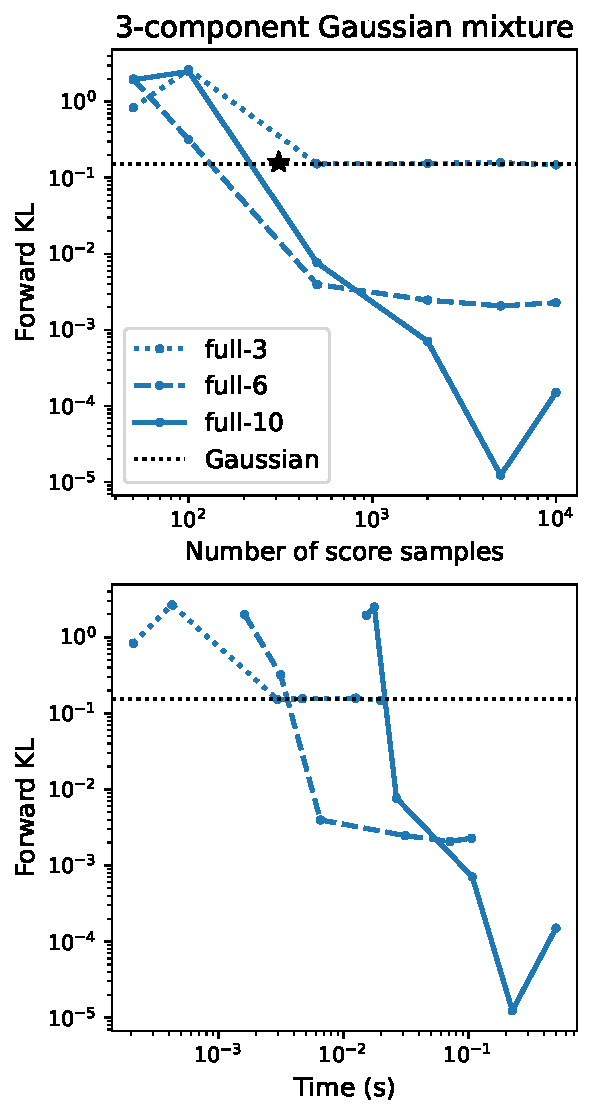
\includegraphics[scale=0.42]{figs/expts-2d/metrics-3gmm_full.pdf}
    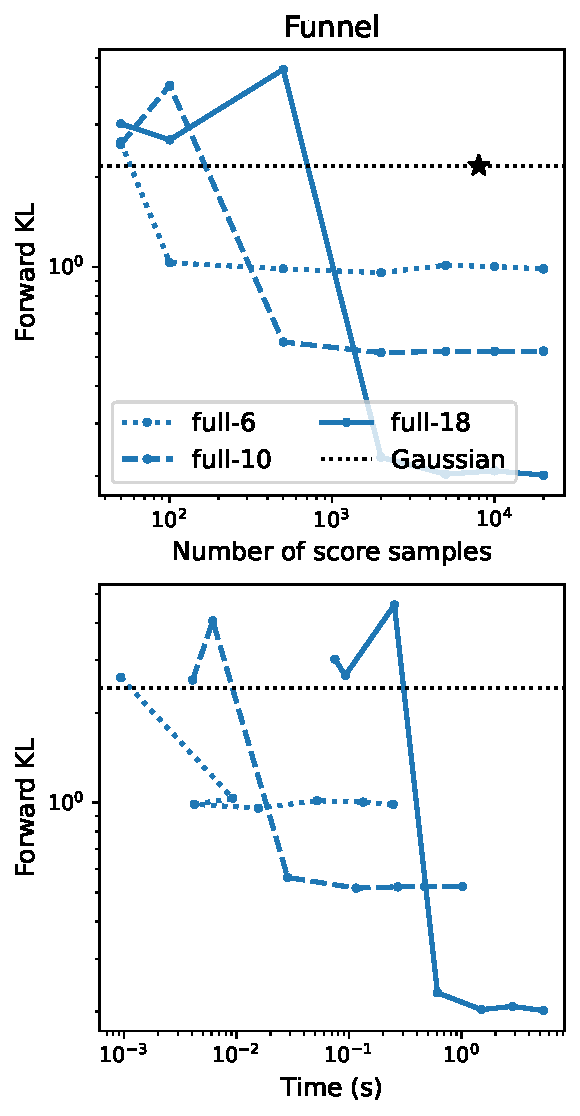
\includegraphics[scale=0.42]{figs/expts-2d/metrics-funnel_full.pdf}
    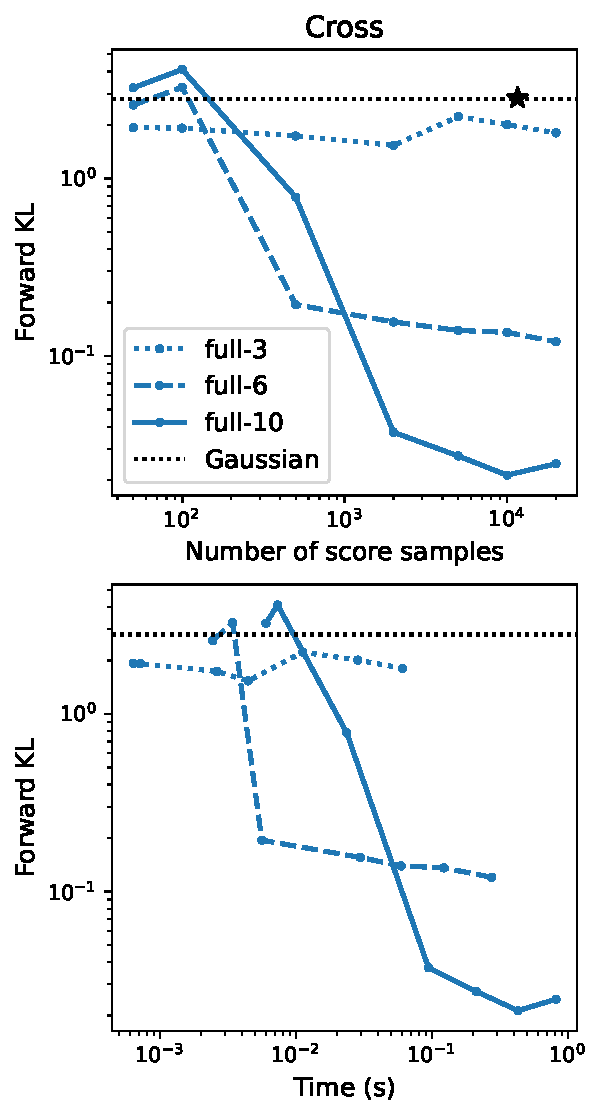
\includegraphics[scale=0.42]{figs/expts-2d/metrics-cross_full.pdf}
    \caption{We compare the number of score evaluations wallclock vs
FKL divergence for the target distributions in
\Cref{fig:2dtargets}: the Gaussian mixture (column 1),
the funnel (column 2), and
the cross (column 3) distributions.
The $K$ used for EigenVI is reported in each figure legend,
where $K=K_1 K_2$.
The black star denotes the number of gradient evaluations for the Gaussian method.
    }
\label{fig:2dtargets-metrics}
\end{figure}

We considered the following synthetic 2D targets:

\begin{itemize}

    \item \textbf{3-component Gaussian mixture:}
    \begin{align*}
    p(z) =
    0.4 \N(z \given [-1,1]^\top,\Sigma)
    +
    0.3 \N(z \given  [1.1,1.1]^\top,0.5I)
    +
    0.3 \N(z \given [-1,-1]^\top,0.5I),
\end{align*}
where we define
$\Sigma =
\begin{bmatrix}
    2 & 0.1 \\
    0.1 & 2 \\
\end{bmatrix}$.


\item \textbf{Funnel distribution with $\sigma^2=1.2$:}
\begin{align*}
    p(z) = \N(z_1 \given 0, \sigma^2) \N(z_2 \given 0, \exp(z_1/2)).
\end{align*}

\item \textbf{ Cross distribution:}
\begin{align*}
    p(z) =
    \tfrac{1}{4} \N(z \given [0,2]^\top,\Sigma_1)
    +
     \tfrac{1}{4} \N(z \given [-2,0]^\top,\Sigma_2)
    +
     \tfrac{1}{4} \N(z \given  [2,0]^\top,\Sigma_2)
    +
     \tfrac{1}{4} \N(z \given  [0,-2]^\top,\Sigma_1),
\end{align*}
where
$\Sigma_1 = \begin{bmatrix}
0.15^{0.9} & 0 \\ 0 & 1
\end{bmatrix}$
and
$\Sigma_2 = \begin{bmatrix}
    1 & 0 \\
0 & 0.15^{0.9}
\end{bmatrix}$.

\end{itemize}

These experiments were conducted without standardization with a Gaussian VI estimate.
The EigenVI proposal distribution $\pi$ used was a $\text{uniform}([-9,9])$ distribution.

In  \Cref{fig:5dtargetdensity}, we run EigenVI for increasing numbers of importance samples $B$
and report the resulting forward KL divergence.
The blue curves denote variational families with different $K_1=K_2=K$ values used,
i.e., 3, 6, and 10 (resulting in a total
number of basis functions of $3^2$, $6^2$, and $10^2$).
In the bottom row of the plot, we also show wall clock timings (computed without parallelization)
to show how the cost grows with the increase in the number of basis functions and importance samples.
The horizontal dotted line denotes the result from batch and match VI,
which fits a Gaussian via score matching; here a batch size of 16 was used
and a learning rate of $\lambda_t = \tfrac{BD}{t+1}$.

The black star denotes the number of score evaluations used by the Gaussian
VI method.


\subsection{Sinh-arcsinh targets}
\label{ssec-sinh}

The sinh-arcsinh normal distribution \citep{jones2009sinh,jones2019sinh}
has parameters $s \in \reals^D, \tau \in \reals_+^D, \Sigma \in \mathbb{S}_{++}$;
it is induced by transforming a
Gaussian $Z_0 \sim \N(0, \Sigma)$ to $Z = \mathcal{S}_{s,\tau}(Z_0)$,
where
\begin{align}
\mathcal{S}_{s,\tau}(z) :=
    [S_{s_1,\tau_1}(z_1), \ldots, S_{s_D,\tau_D}(z_D)]^\top,
    \quad
S_{s_d,\tau_d}(z_d) := \sinh\left(\tfrac{1}{\tau_d} \sinh^{-1}(z_d) + \tfrac{s_d}{\tau_d}\right).
\end{align}
Here $s_d$ controls the amount of skew in the $d$th dimension,
and $\tau_d$ controls the tail weight in that dimension.
When $s_d\!=\!{0}$ and $\tau_d\!=\!{1}$ in all dimensions $d$, the distribution is Gaussian. % the Gaussian distribution.



The sinh-arcsinh normal distribution has the following density:
\begin{align}
p(z; s, \tau, \Sigma)
    = [(2\pi)^D |\Sigma|]^{-\frac{1}{2}}
    \prod_{d=1}^D
    \left\{
        (1 + z_d^2)^{-\frac{1}{2}}
\tau_d \, C_{s_d, \tau_d}(z_d)
    \right\}
\exp\left(-\frac{1}{2} S_{s,\tau}(z)^\top \Sigma^{-1} S_{s,\tau}\right),
\end{align}
where we define the functions
\begin{align}
    C_{s_d,\tau_d}(z_d) := (1 + S_{s_d,\tau_d}^2(z))^{\frac{1}{2}},
\end{align}
and
\begin{align}
    \quad
    S_{s_d,\tau_d}(z_d) := \sinh(\tau_d \sinh^{-1}(z_d) - s_d),
    \quad
    S_{s,\tau}(z) =
    [S_{s_1,\tau_1}(z_1), \ldots, S_{s_D,\tau_D}(z_D)]^\top.
\end{align}

We constructed 3 targets in 2 dimensions and 3 targets in 5 dimensions,
each with varying amounts of non-Gaussianity.
The details of each target are below.
In all experiments, EigenVI was applied with standardization,
where a Gaussian was fit using batch and match VI with a batch size of 16
and a learning rate $\lambda_t = \tfrac{BD}{t+1}$.
%


For all experiments, we used a proposal distribution $\pi$
that was uniform on $[-5,5]^2$.

\begin{figure}[t]
    \centering
    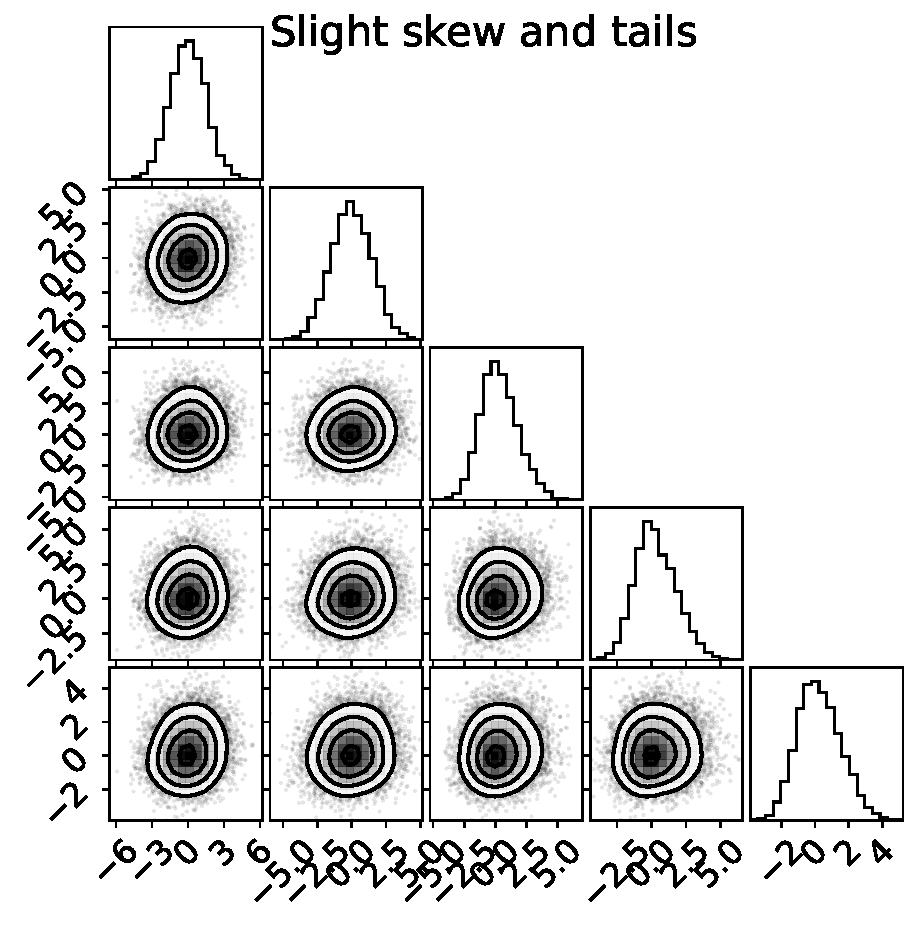
\includegraphics[scale=0.28]{figs/expts-2d/sinh_5D_target1v2.pdf}
    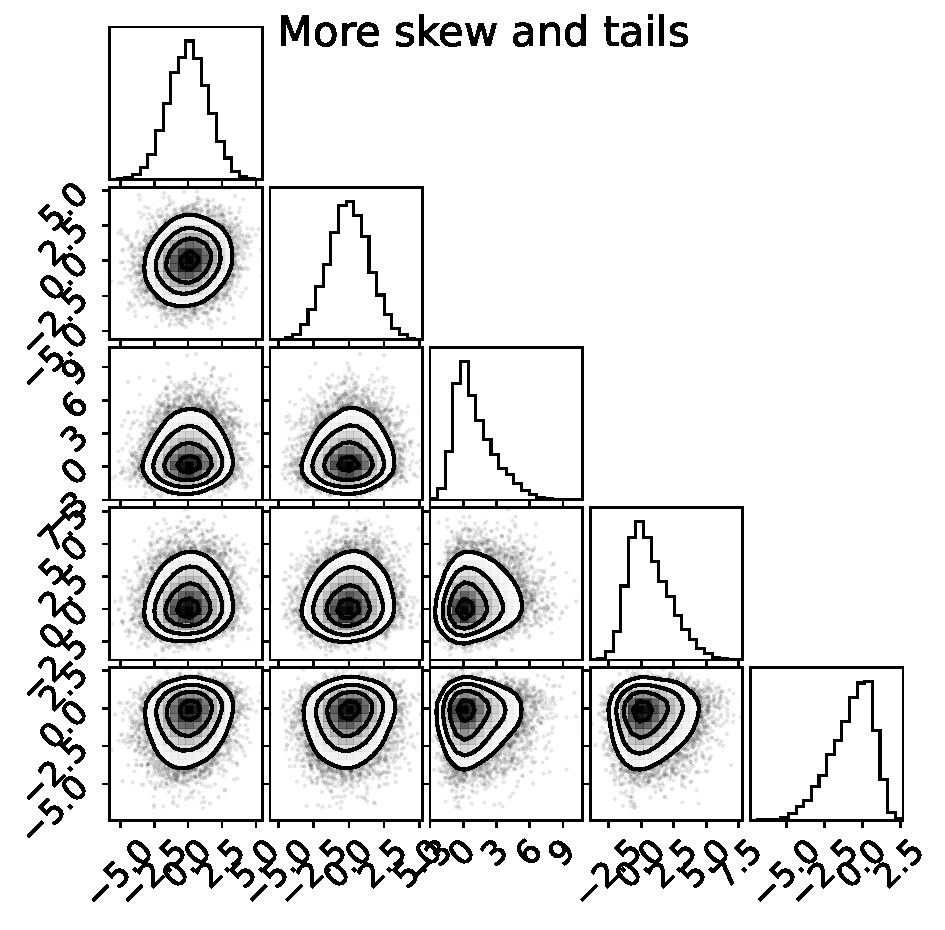
\includegraphics[scale=0.28]{figs/expts-2d/sinh_5D_target2v2.pdf}
    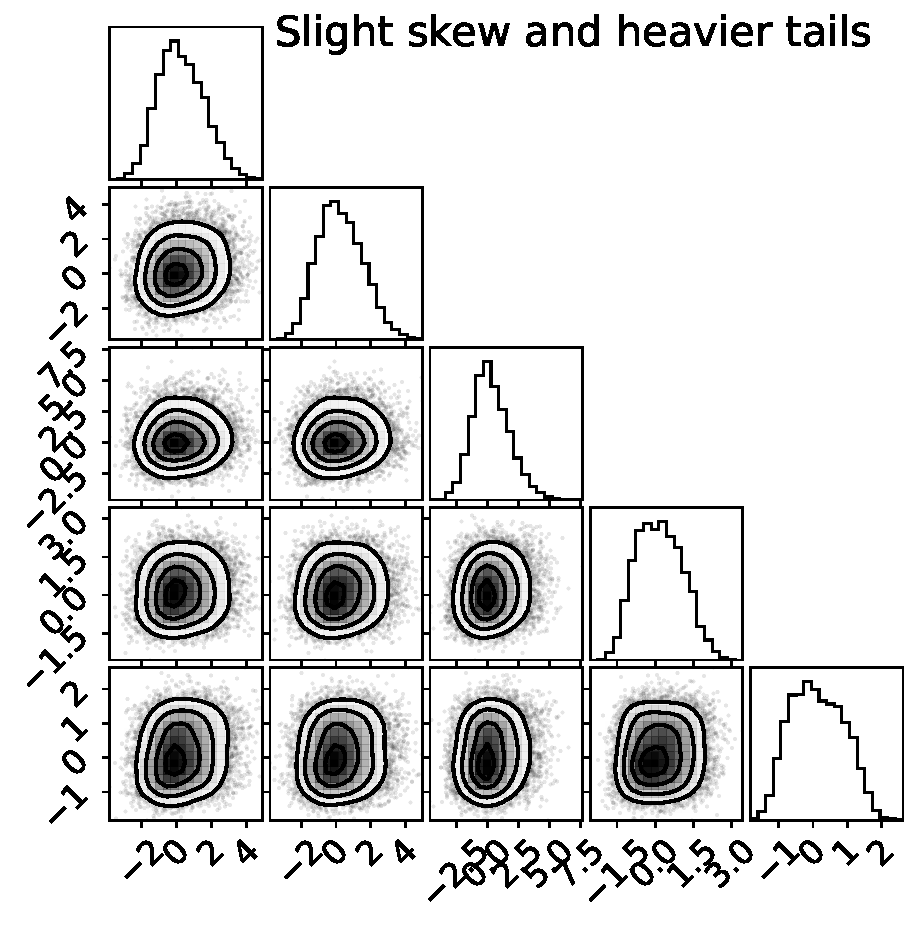
\includegraphics[scale=0.28]{figs/expts-2d/sinh_5D_target3v2.pdf}
    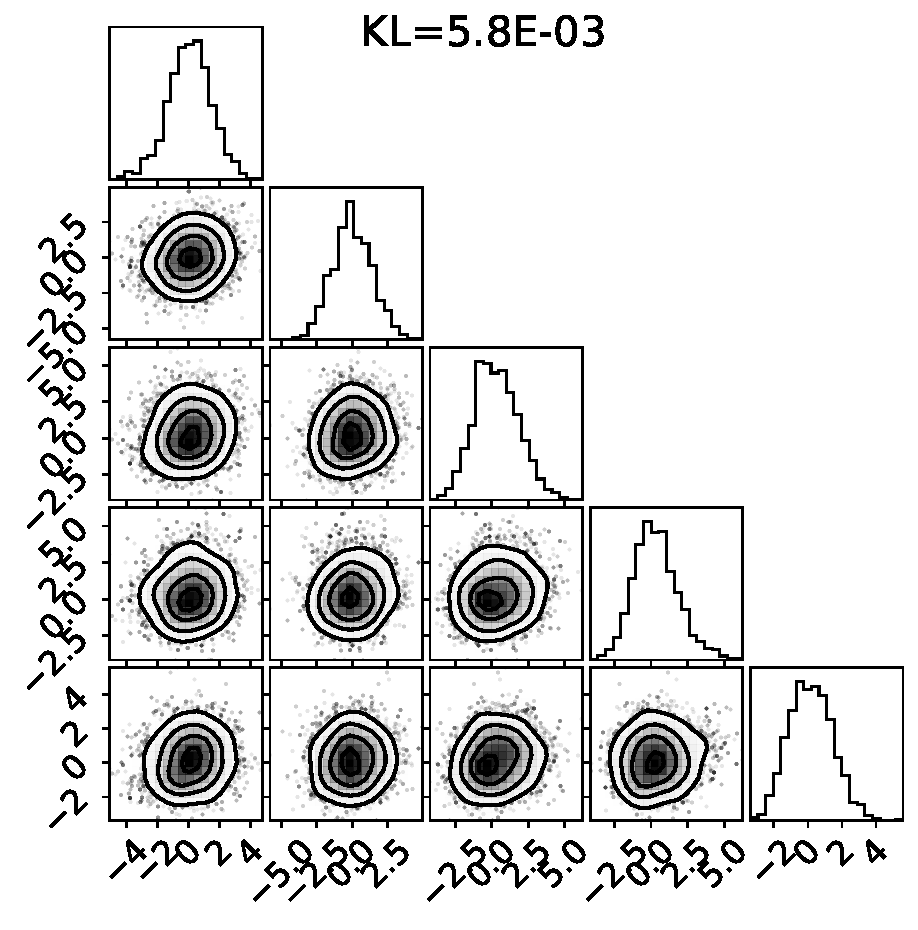
\includegraphics[scale=0.28]{figs/expts-2d/sinh_5D_target1-fit.pdf}
    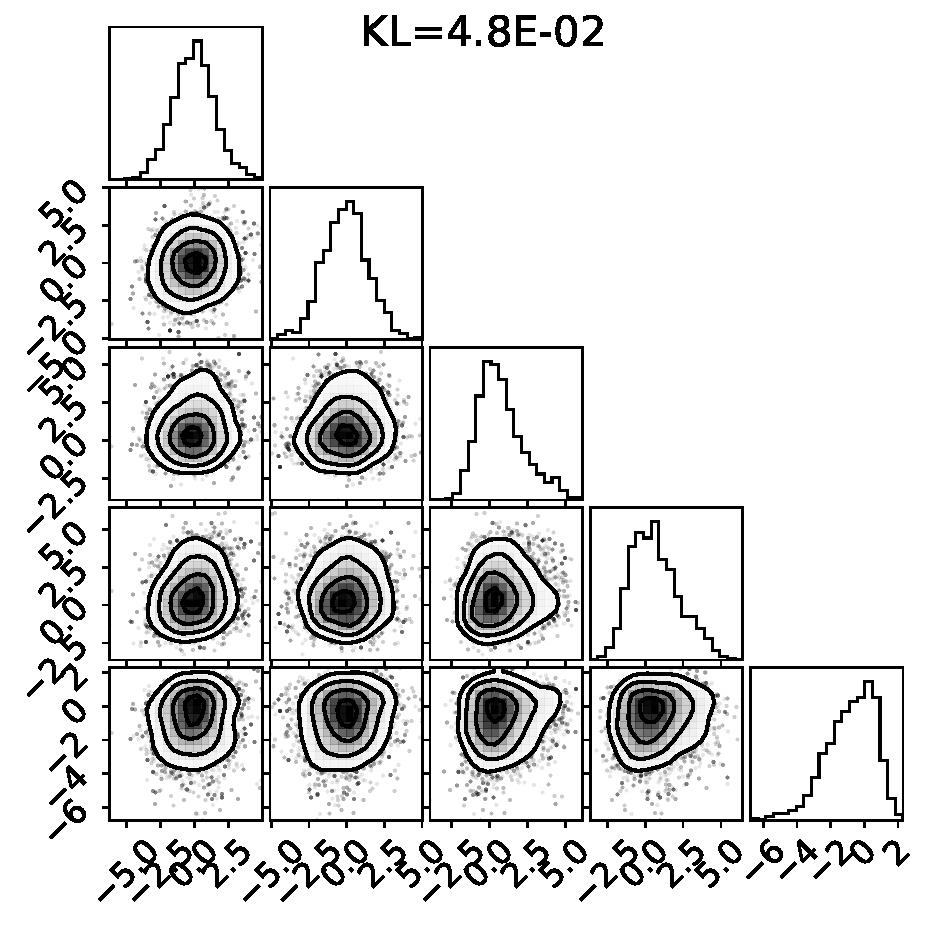
\includegraphics[scale=0.28]{figs/expts-2d/sinh_5D_target2-fit.pdf}
    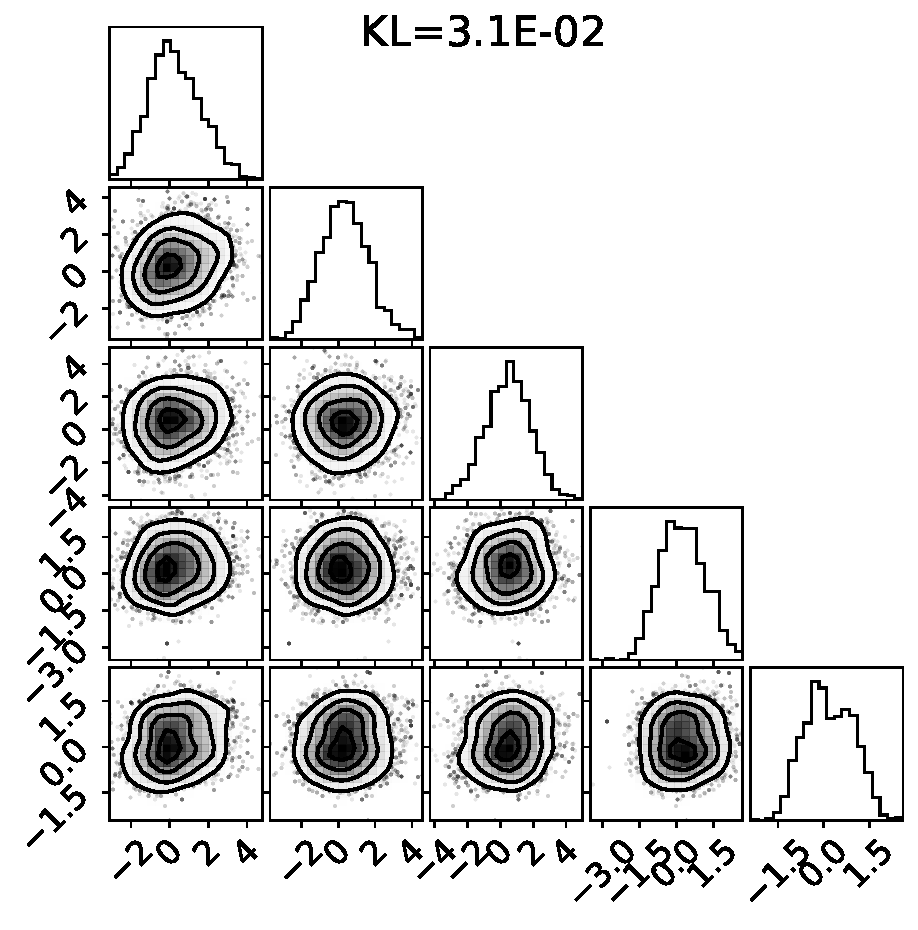
\includegraphics[scale=0.28]{figs/expts-2d/sinh_5D_target3-fit.pdf}
\caption{Targets (top) for the 5D sinh-arcsinh normal distribution example
and EigenVI fits (bottom) with the KL divergence in the figure title.}
\label{fig:5dtargetdensity}
\end{figure}

\paragraph{2D sinh-arcsinh normal experiment}
For $D=2$ (\Cref{subfig:sinh2D}), we consider the
\emph{slight skew and tails target} with parameters
$s=[0.2,0.2], \tau = [1.1,1.1]$,
the \emph{more skew and tails target} with
$s=[0.2,0.5], \tau = [1.1,1.1]$,
and \emph{the slight skew and heavier tails} with
$s=[0.2,0.2], \tau = [1.4,1.1]$.
Note that $s=[0,0], \tau=[1,1]$ recovers the multivariate Gaussian.
%
These three target are visualized in
\Cref{fig:sinh2dtargets}.

\paragraph{5D sinh-archsinh normal experiment}


We constructed three targets $P_1$ (slight skew and tails), $P_2$ (more skew and tails),
and $P_3$ (slight skew and heavier tails) each with
\begin{align}
    \Sigma =
\begin{bmatrix}
    2.2 & 0.3 & 0   & 0   & 0.3 \\
    0.3 & 2.2 & 0   & 0   & 0 \\
    0   & 0   & 2.2 & 0.3 & 0 \\
    0   & 0   & 0.3 & 2.2 & 0 \\
    0.3 & 0   & 0   & 0   & 2.2 \\
\end{bmatrix}.
\end{align}
The skew and tail weight parameters used were:
$s_1 = [0.,0.,0.2,0.2,0.2]; \tau_1 = [1., 1., 1., 1., 1.1]$,
$s_2 = [0.0,0.0,0.6,0.4,-0.5]; \tau_2 = [1., 1., 1., 1., 1.1]$,
and
$s_3 = [0.2,0.2,0.2,0.2,0.2]; \tau_3 = [1.1, 1.1, 1., 1.4, 1.6]$.
See \Cref{fig:5dtargetdensity} for a visualization of the marginals of each target distribution.
In the second row, we show examples of resulting EigenVI fit (visualized using samples from $q$)
from $B=20{,}000$ and $K=10$.


\subsection{Posteriordb experiments}
\label{ssec:pdb}

We consider 8 real data targets from \texttt{posteriordb}, a suite of benchmark
Bayesian models for real data problems.
In \Cref{table:posteriordb}, we summarize the models considered in the study.
These target distributions are non-Gaussian, typically with some skew or different tails.
To access the log target probability and their gradients, we used the
BridgeStan library \citep{roualdes2023bridgestan}, which by default transforms the target
to be supported on $\reals^D$.

For all experiments, we fixed the number of importance samples to be
$B=40{,}000$; to construct the EigenVI matrix $M$, the computations were parallelized
over the samples.
These experiments were repeated over 5 random seeds, and we report the mean and standard errors in
\Cref{fig:posteriordb}; for lower dimensions, there was little variation between runs.

The target distributions were standardized using a Gaussian fit from score matching
before applying EigenVI.
In most cases, the proposal distribution $\pi$ was chosen to be uniform over $[-6,6]^D$.
For the models \texttt{8-schools},
which has a longer tail, we used a multivariate Gaussian proposal with zero mean
and a scaled diagonal covariance $\sigma I$, with $\sigma = 3^2$.

\begin{table}
\caption{Summary of \texttt{posteriordb} models}
\label{table:posteriordb}
    \centering
    \small
\begin{tabular}{ccc}
    \toprule
    Name & Dimension & Model description \\
    \midrule
    \texttt{kidscore} & 3 & linear model with a Cauchy noise prior \\
   % \texttt{earn-height} & 3 & linear model with uniform prior \\
    \texttt{sesame} & 3 & linear model with uniform prior \\
    \texttt{gp\_regr} & 3 & Gaussian process regression with squared exponential kernel \\
    \texttt{garch11} & 4 & generalized autoregressive conditional heteroscedastic model \\
    \texttt{logearn} & 4 & log-log linear model with multiple predictors \\
    \texttt{arK-arK} & 7 & autoregressive model for time series \\
    \texttt{logmesquite} & 7 & multiple predictors log-log model  \\
    %\texttt{bball-hmm} & 8 & hidden Markov model with exponential distribution emissions \\
    \texttt{8-schools} & 10 & non-centered hierarchical model for 8-schools \\
    \bottomrule
\end{tabular}
\end{table}


\begin{figure}
    \centering
    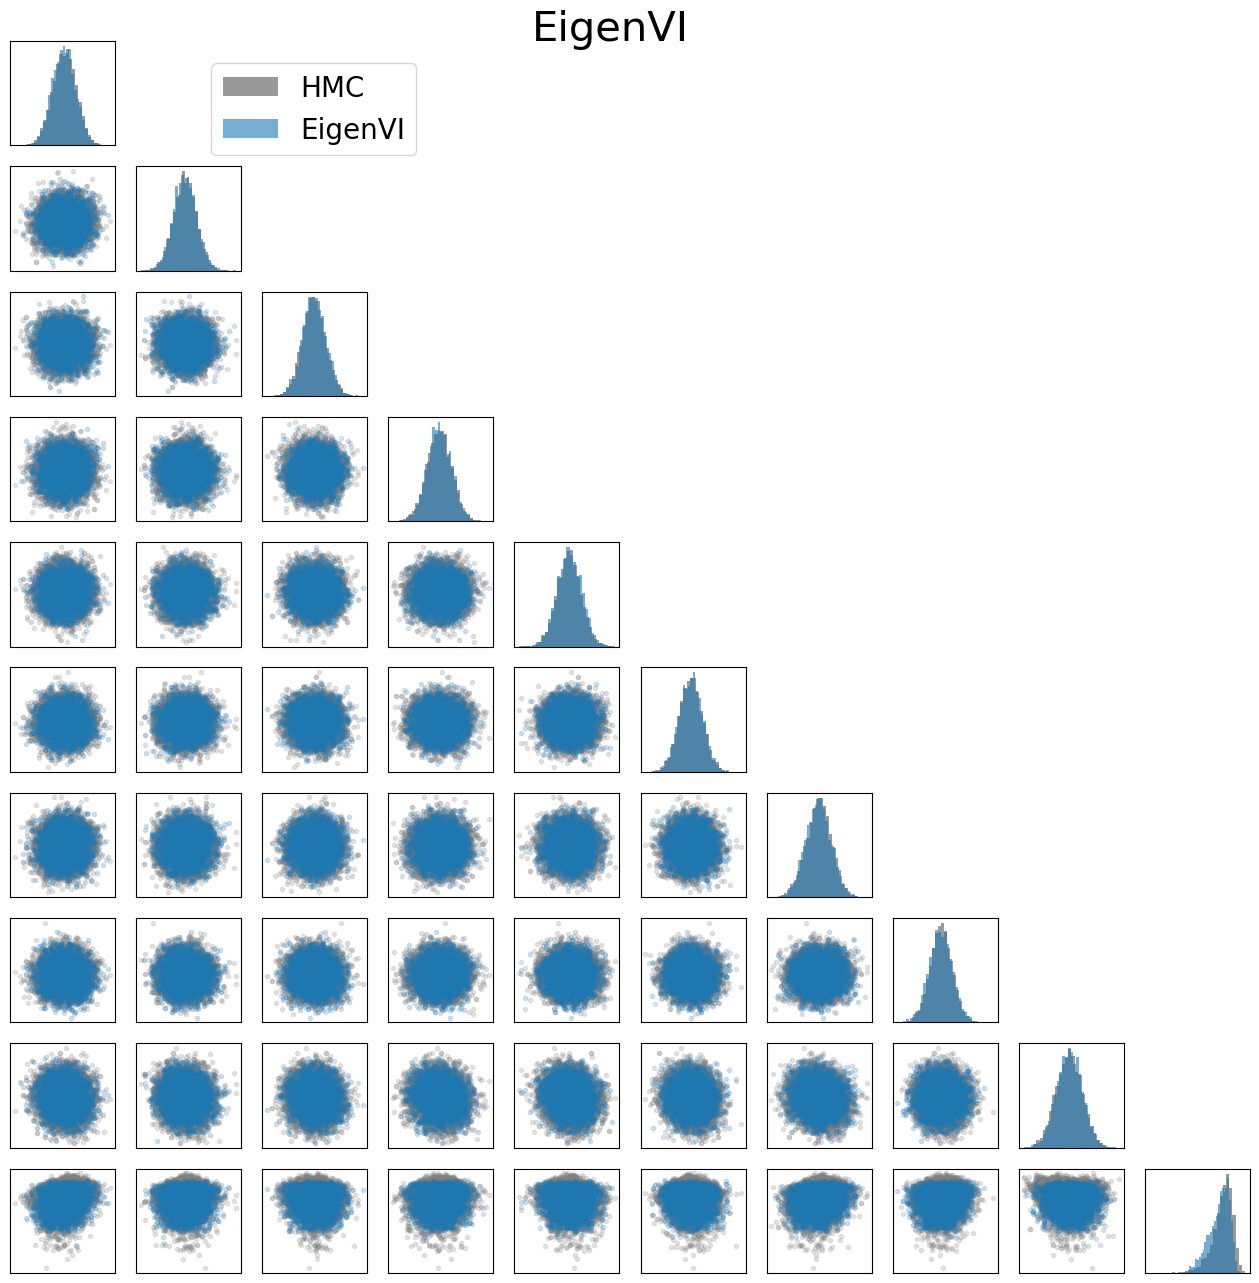
\includegraphics[scale=0.23]{figs/expts-pdb/PDB_85_corner_eigenvi.png}
    \\
    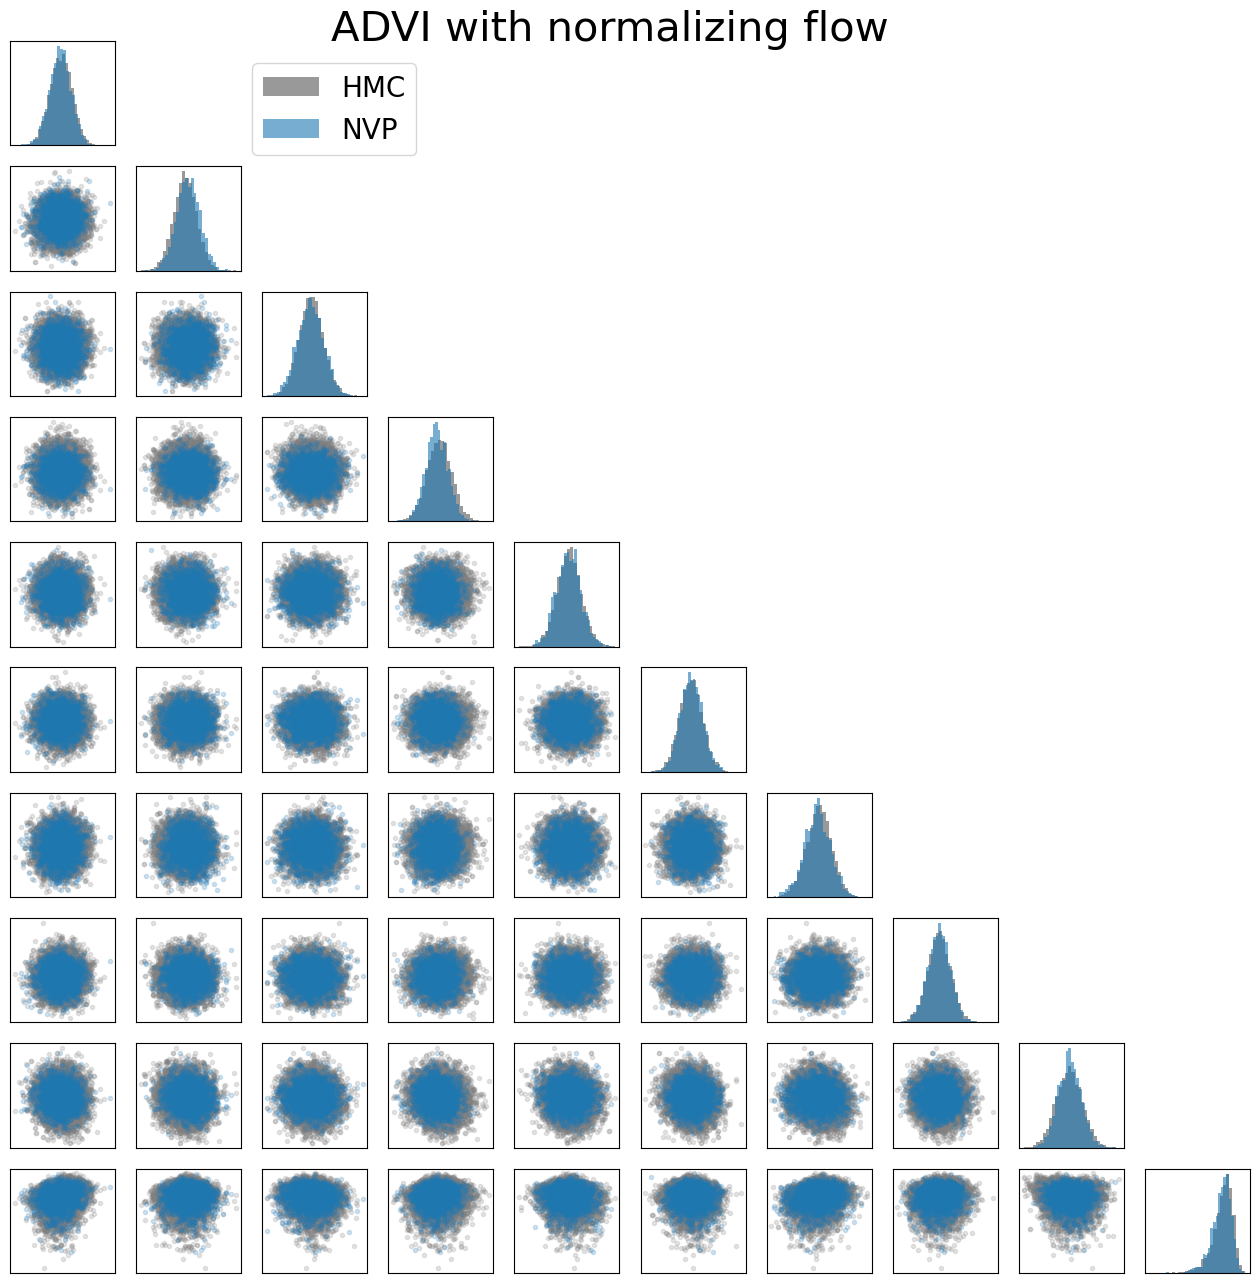
\includegraphics[scale=0.23]{figs/expts-pdb/PDB_85_corner_flows.png}
    \\
    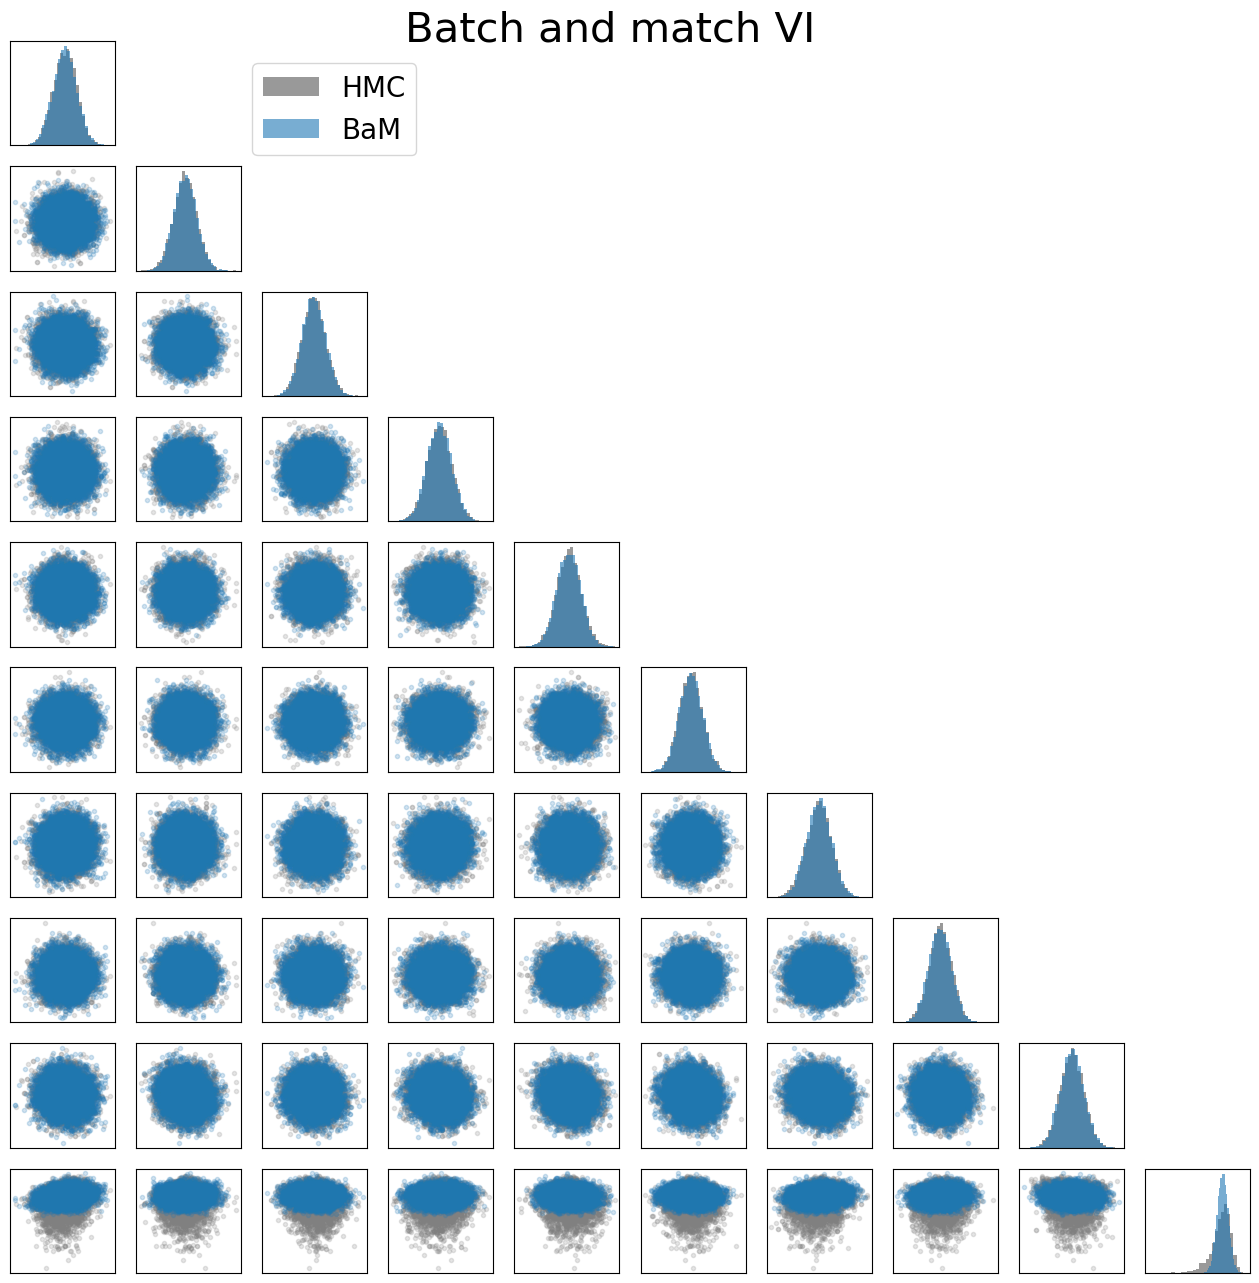
\includegraphics[scale=0.23]{figs/expts-pdb/PDB_85_corner_bam.png}
    \caption{Comparison of EigenVI, normalizing flow,
    and Gaussian score-based BBVI methods on
\texttt{8schools}.
    }
\label{fig:8schools:corner}
\end{figure}

\begin{figure}
    \centering
    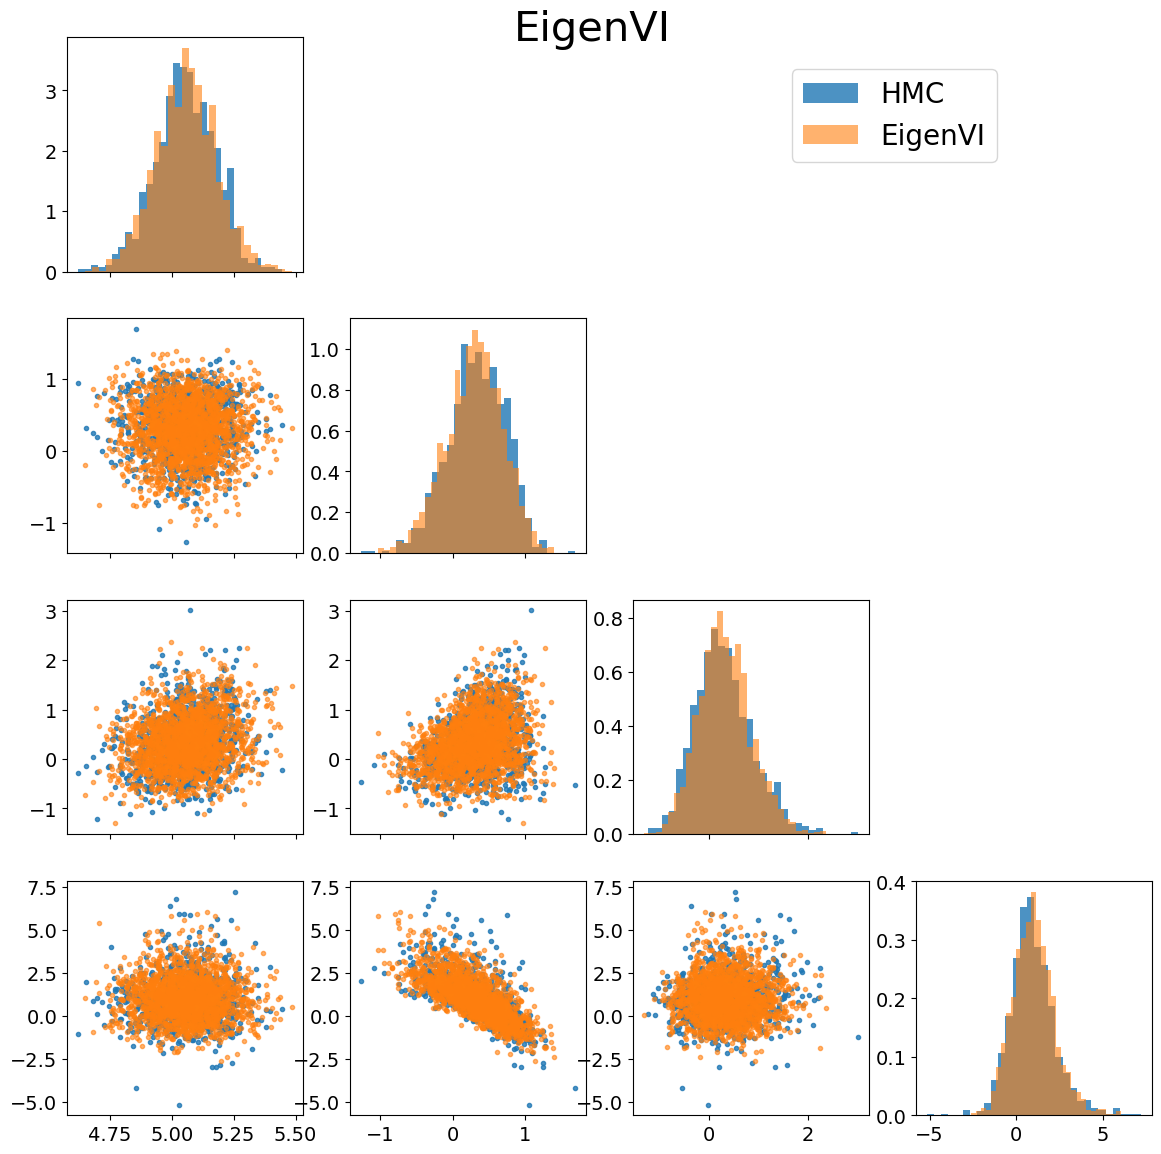
\includegraphics[scale=0.23]{figs/expts-pdb/PDB_99_samples_eigenvi.png}
    \\
    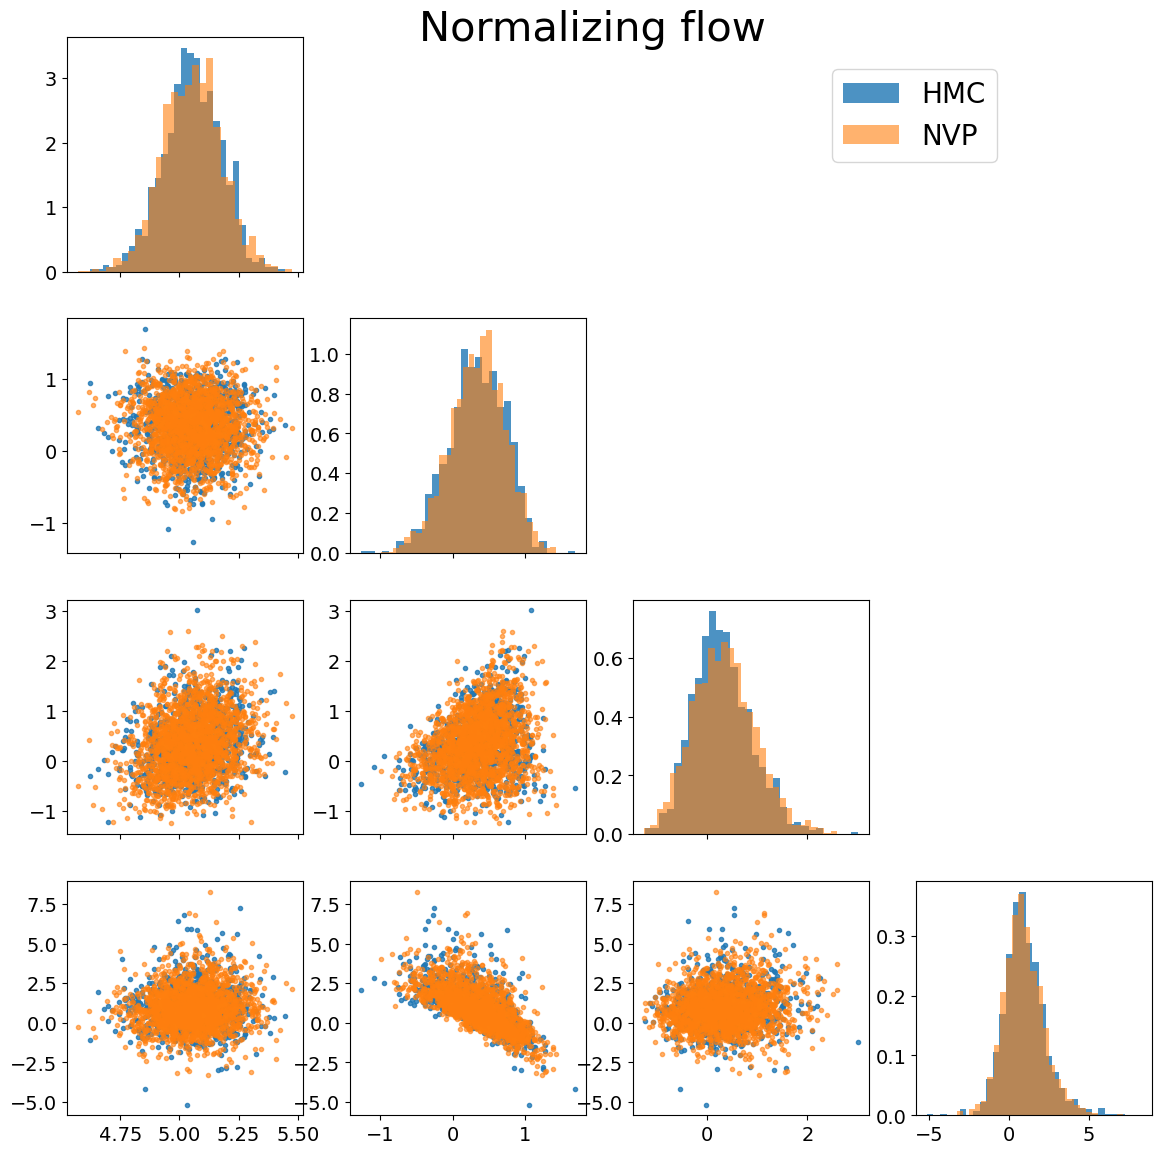
\includegraphics[scale=0.23]{figs/expts-pdb/PDB_99_samples_flow.png}
    \\
    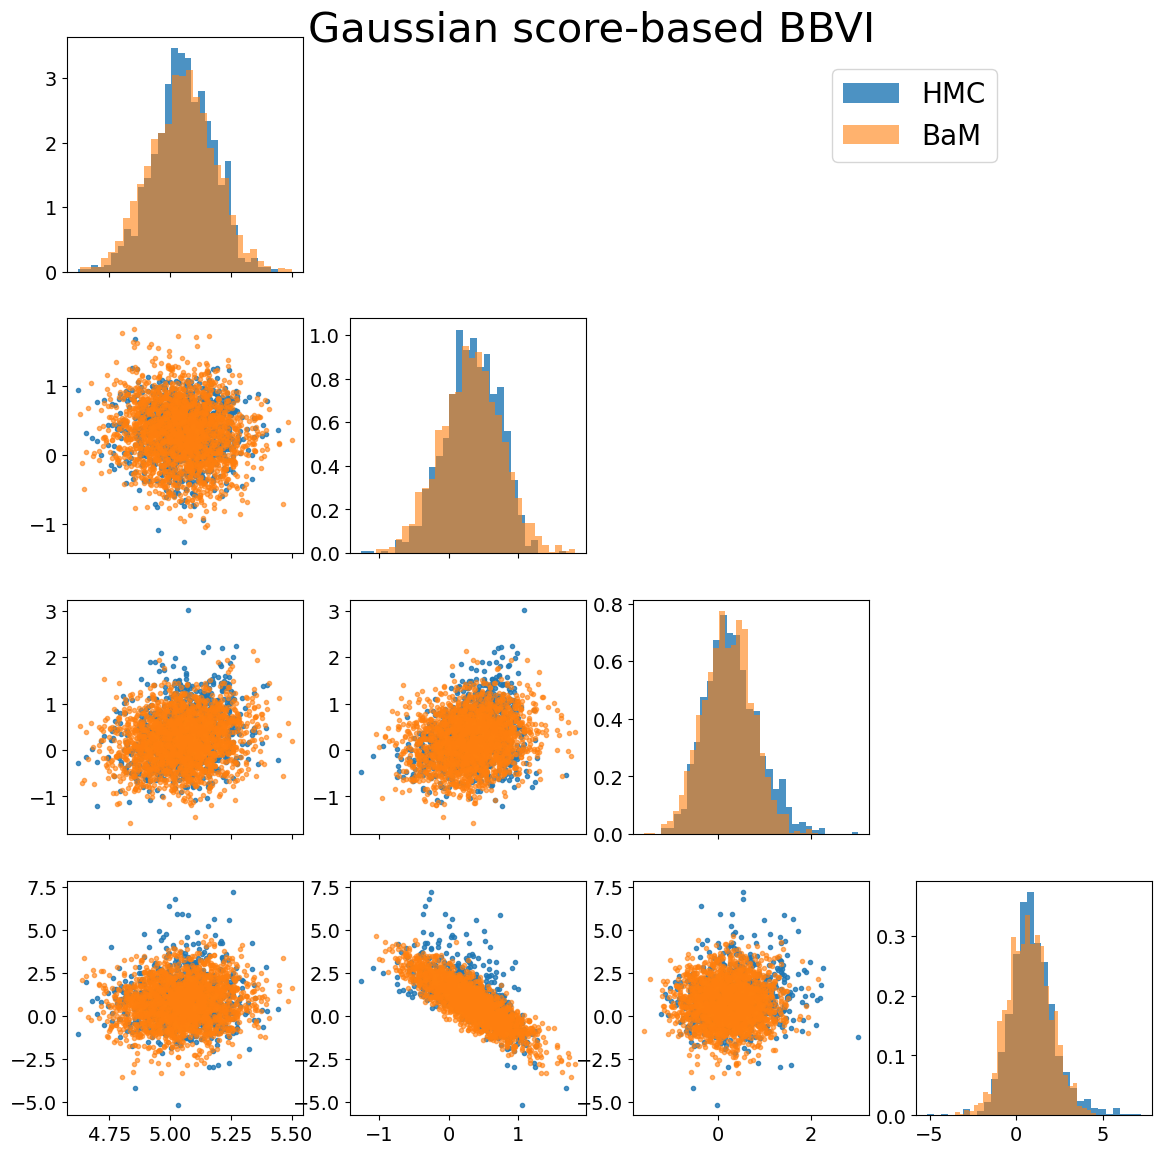
\includegraphics[scale=0.23]{figs/expts-pdb/PDB_99_samples_bam.png}
    \caption{Comparison of EigenVI, normalizing flow,
    and Gaussian score-based BBVI methods on
\texttt{garch11}.
Note that the Gaussian approximation over/underestimates the tails,
while the more expressive families fit the tails better.
    }
\label{fig:garch11:corner}
\end{figure}


For the Gaussian score matching (GSM) method \citep{modi2023},
we chose a batch size of 16 for all experiments. We generally found the
results were not too sensitive in comparison to other batch sizes of 4,8, and 32.
For the batch and match (BaM) method \citep{cai2024}, we chose a batch size of 16.
The learning rate was fixed at
$\lambda_t = \tfrac{BD}{t+1}$, which was a recommended schedule for non-Gaussian targets.

For all ELBO optimization methods (full covariance Gaussian family and normalizing flow family),
we used Adam to optimize the ELBO.
We performed a grid search over the learning rate
$0.01, 0.02, 0.05, 0.1$ and batch size $B=4,8,16,32$.
For the normalizing flow model,
we used a real NVP \citep{dinh2016density}
with 8 layers and 32 neurons.
We found empirically that the computational of the scores was unreliable~\cite{kohler2021smooth,
Zeghal2022npe};
hence we do not show their Fisher divergence in \Cref{fig:posteriordb}.


In \Cref{fig:8schools:corner}
and
\Cref{fig:garch11:corner},
we show the corner plots that compare an EigenVI fit, a normalizing flow fit, and a Gaussian fit
(BaM).
In each plot, we plot the samples from the variational distribution against
samples from Hamiltonian Monte Carlo.
We observe that the two more expressive families EigenVI and the normalizing flow
are able to model the tails of the distribution better than the Gaussian fit.

%\end{document}



\section{Broader impacts}

EigenVI adds to the literature on BBVI,
which has been an important line of work for developing automated, approximate
Bayesian inference methods.
In terms of positive societal impacts, Bayesian models are used
throughout the sciences and engineering, and advances in fast
and automated inference will aid in advances in these fields.
In terms of negative societal impacts, advances in BBVI could be
used to train generative models with malicious or unintended uses.



%%%%%%%%%%%%%%%%%%%%%%%%%%%%%%%%%%%%%%%%%%%%%%%%%%%%%%%%%%%%




\end{document}

%%% Local Variables:
%%% mode: latex
%%% TeX-master: t
%%% End:
